\documentclass[14pt,a4paper]{article}

% ------------------------------------------------------------
% Packages
% ------------------------------------------------------------
\usepackage[margin=1in]{geometry}
\usepackage{amsmath,amssymb,bm}
\usepackage{booktabs}
\usepackage{array}
\usepackage{siunitx}
\usepackage{graphicx}
\graphicspath{{./}}
\usepackage{float}
\usepackage{xcolor}
\usepackage{hyperref}
\usepackage{caption}
\usepackage{subcaption}
\usepackage{fancyhdr}

\hypersetup{
    colorlinks=true,
    linkcolor=blue,
    urlcolor=blue,
    citecolor=blue
}

\sisetup{round-mode=places,round-precision=4}

% ------------------------------------------------------------
% Convenience macros
% ------------------------------------------------------------
\newcommand{\dd}{\,\mathrm{d}}
\newcommand{\grad}{\nabla}
\newcommand{\vect}[1]{\begin{Bmatrix}#1\end{Bmatrix}}
\newcommand{\mat}[1]{\begin{bmatrix}#1\end{bmatrix}}

\fancyhf{}
\fancyhead[L]{CE526 Assignment 5}
\fancyhead[R]{Imran Shahriar - 2735835}
\renewcommand{\headrulewidth}{0.4pt}
\fancyfoot[C]{\thepage}
\fancypagestyle{plain}{%
\fancyhf{}
\fancyhead[L]{CE526 Assignment 5}
\fancyhead[R]{Imran Shahriar - 2735835}
\renewcommand{\headrulewidth}{0.4pt}
\fancyfoot[C]{\thepage}}
\pagestyle{fancy}

\begin{document}

% ============================================================
% Title Page
% ============================================================
\begin{titlepage}
    \begin{flushright}
        {\large \today\par}
    \end{flushright}

    \vspace*{0.5cm}

    \begin{center}
        
\includegraphics[width=0.42\textwidth]{images/metu_logo.jpg}\par
        \vspace{0.7cm}
        {\huge CE526 Assignment 5\par}
        \vspace{0.45cm}
        {\Large Finite Element Method\par}
        \vspace{0.3cm}
        {\Large Spring Semester 2025--2026\par}
 \vspace{0.3cm}
\end{center}

\vspace{0.9cm}

\noindent
\begin{minipage}[t]{0.48\textwidth}
    \raggedright
    {\Large \textbf{Submitted By}\par}
    \vspace{0.2cm}
    {\large Imran Shahriar\par}
    {\large 2735835\par}
    {\large MSc. in Structural Engineering\par}
\end{minipage}
\hfill
\begin{minipage}[t]{0.48\textwidth}
    \raggedleft
    {\Large \textbf{Submitted To}\par}
    \vspace{0.2cm}
    {\large Prof. Ayşegül Askan Gündoğan\par}
\end{minipage}

\vspace{0.5cm}

\begin{center}
\textbf{\large GitHub Repository:} 
\href{https://github.com/ImranMETU/CE526_Assignment5}{\url{https://github.com/ImranMETU/CE526_Assignment5}}
\end{center}
    \vfill
\end{titlepage}
\hypersetup{pageanchor=true}



\section{Problem Statement}

The problem is a scalar two-dimensional boundary-value problem on an L-shaped domain. The governing equation is
\begin{equation}
    -\Delta u = 1 \qquad \text{in } \Omega,
\end{equation}
with homogeneous Dirichlet boundary condition on all boundaries,
\begin{equation}
    u = 0 \qquad \text{on } \Gamma.
\end{equation}

The origin is taken at the re-entrant corner. The positive $x$-axis points to the right and the positive $y$-axis points upward. The domain is interpreted as
\begin{equation}
    \Omega = [-2,2]\times[0,2] \;\cup\; [-2,0]\times[-2,0].
\end{equation}

The assignment is solved twice:
\begin{enumerate}
    \item Part A: using 24 linear triangular elements obtained by splitting each unit square into two triangles.
    \begin{figure}[H]
    \centering
    \begin{minipage}{0.48\textwidth}
        \centering
        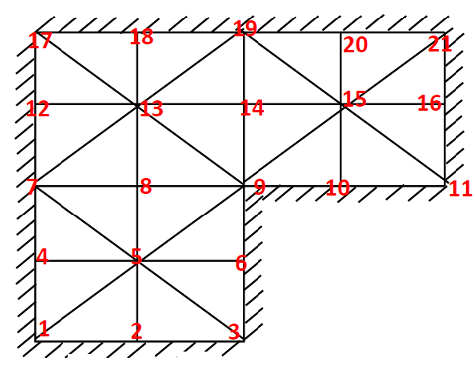
\includegraphics[width=\textwidth]{images/partA_nodenumbering.png}
        \caption*{(a) Part A node numbering.}
    \end{minipage}
    \hfill
    \begin{minipage}{0.48\textwidth}
        \centering
        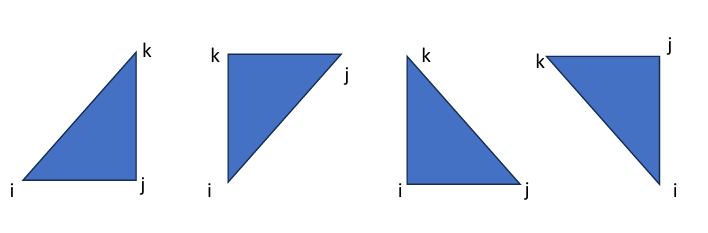
\includegraphics[width=\textwidth]{images/partA_elementshapes.png}
        \caption*{(b) Part A element shapes.}
    \end{minipage}
    \caption{Part A triangular discretization: node numbering and element-shape definition.}
    \label{fig:parta_numbering_shapes}
    \end{figure}

    \item Part B: using 12 bilinear rectangular elements, each with size $1\times 1$.
    \begin{figure}[H]
    \centering
    \begin{minipage}{0.48\textwidth}
        \centering
        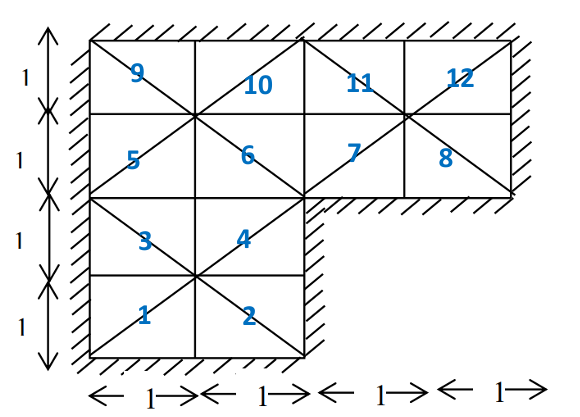
\includegraphics[width=\textwidth]{images/partB_elementnumbering.png}
        \caption*{(a) Part B node and element numbering.}
    \end{minipage}
    \hfill
    \begin{minipage}{0.48\textwidth}
        \centering
        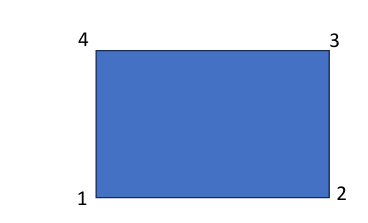
\includegraphics[width=\textwidth]{images/partB_elementshapes.png}
        \caption*{(b) Part B element shapes.}
    \end{minipage}
    \caption{Part B rectangular discretization: numbering scheme and bilinear element shapes.}
    \label{fig:partb_numbering_shapes}
    \end{figure}
\end{enumerate}

The physical interpretations include transverse deformation of a membrane, torsion of a solid shaft, and two-dimensional heat conduction.

\section{Finite Element Formulation}

\subsection{Weak Form}

The standard scalar diffusion/Poisson problem is
\begin{equation}
    -\grad\cdot(k\grad u)=f \qquad \text{in } \Omega.
\end{equation}

For this assignment,
\begin{equation}
    k=1, \qquad f=1.
\end{equation}

Multiplying the strong form by a test function $v$ and integrating over the domain gives
\begin{equation}
    \int_{\Omega} -v\,\grad\cdot(k\grad u)\dd\Omega
    =
    \int_{\Omega} fv\dd\Omega.
\end{equation}

After integration by parts, the weak form becomes
\begin{equation}
    \int_{\Omega} k\grad u\cdot \grad v\dd\Omega
    =
    \int_{\Omega} fv\dd\Omega
    +
    \int_{\Gamma_q} \bar q v\dd\Gamma.
\end{equation}

Since this problem has only homogeneous Dirichlet boundary conditions, there is no prescribed Neumann flux term in the load vector. Therefore,
\begin{equation}
    \int_{\Omega} \grad u\cdot \grad v\dd\Omega
    =
    \int_{\Omega} v\dd\Omega.
\end{equation}

The finite element system has the form
\begin{equation}
    KU=F.
\end{equation}

\subsection{Linear Triangular Element}

For a 3-node linear triangular element,
\begin{equation}
    u_h(x,y)=N_1u_1+N_2u_2+N_3u_3.
\end{equation}

The shape functions are
\begin{equation}
    N_i(x,y)=\frac{1}{2A_e}\left(\alpha_i+\beta_i x+\gamma_i y\right),
\end{equation}
where $A_e$ is the element area. For local nodes $(1,2,3)$ ordered counterclockwise,
\begin{align}
    \beta_1 &= y_2-y_3, & \gamma_1 &= x_3-x_2,\\
    \beta_2 &= y_3-y_1, & \gamma_2 &= x_1-x_3,\\
    \beta_3 &= y_1-y_2, & \gamma_3 &= x_2-x_1.
\end{align}

The element stiffness matrix is
\begin{equation}
    K_{ij}^{(e)}=\frac{k}{4A_e}\left(\beta_i\beta_j+\gamma_i\gamma_j\right).
\end{equation}

For this assignment, $k=1$ and every triangular element is a unit right triangle with
\begin{equation}
    A_e=\frac{1}{2}.
\end{equation}
Therefore,
\begin{equation}
    K_{ij}^{(e)}=\frac{1}{2}\left(\beta_i\beta_j+\gamma_i\gamma_j\right).
\end{equation}

For constant source $f=1$, the element force vector is
\begin{equation}
    F^{(e)}=\frac{fA_e}{3}\vect{1\\1\\1}
    =
    \frac{1}{6}\vect{1\\1\\1}.
\end{equation}

\subsection{Bilinear Rectangular Element}

For a 4-node bilinear rectangular element, the local node order is
\begin{equation}
    1=\text{BL}, \qquad 2=\text{BR}, \qquad 3=\text{TR}, \qquad 4=\text{TL}.
\end{equation}

Using local coordinates $(\xi,\eta)$ on a unit square, $0\leq \xi\leq 1$ and $0\leq \eta\leq 1$, the shape functions are
\begin{align}
    N_1 &= (1-\xi)(1-\eta),\\
    N_2 &= \xi(1-\eta),\\
    N_3 &= \xi\eta,\\
    N_4 &= (1-\xi)\eta.
\end{align}

The local stiffness matrix for a $1\times1$ bilinear rectangle with $k=1$ is
\begin{equation}
K^{(e)}=
\mat{
2/3 & -1/6 & -1/3 & -1/6\\
-1/6 & 2/3 & -1/6 & -1/3\\
-1/3 & -1/6 & 2/3 & -1/6\\
-1/6 & -1/3 & -1/6 & 2/3
}.
\end{equation}

For constant source $f=1$, the element force vector is
\begin{equation}
    F^{(e)}=\frac{1}{4}\vect{1\\1\\1\\1}.
\end{equation}

\section{Mesh and Boundary Conditions}

There are 21 nodes. The free nodes are
\begin{equation}
    U_f=\vect{u_5\\u_8\\u_{13}\\u_{14}\\u_{15}}.
\end{equation}

All remaining nodes are boundary nodes and have prescribed value
\begin{equation}
    u=0.
\end{equation}

Thus, after partitioning the system,
\begin{equation}
    K_{ff}U_f+K_{fc}U_c=F_f.
\end{equation}
Since $U_c=0$, the reduced system becomes
\begin{equation}
    K_{ff}U_f=F_f.
\end{equation}

\section{Part A: Linear Triangular Elements}

\subsection{Reduced System}

The assembled reduced stiffness matrix is
\begin{equation}
K_{ff}^{\triangle}=
\mat{
4 & -1 & 0 & 0 & 0\\
-1 & 4 & -1 & 0 & 0\\
0 & -1 & 4 & -1 & 0\\
0 & 0 & -1 & 4 & -1\\
0 & 0 & 0 & -1 & 4
}.
\end{equation}

The reduced force vector is
\begin{equation}
F_f^{\triangle}=
\vect{
4/3\\
2/3\\
4/3\\
2/3\\
4/3
}.
\end{equation}

Therefore,
\begin{equation}
\mat{
4 & -1 & 0 & 0 & 0\\
-1 & 4 & -1 & 0 & 0\\
0 & -1 & 4 & -1 & 0\\
0 & 0 & -1 & 4 & -1\\
0 & 0 & 0 & -1 & 4
}
\vect{u_5\\u_8\\u_{13}\\u_{14}\\u_{15}}
=
\vect{4/3\\2/3\\4/3\\2/3\\4/3}.
\end{equation}

\subsection{Nodal Solution}

Solving the reduced system gives
\begin{equation}
U_f^{\triangle}=\vect{
0.435897\\
0.410256\\
0.538462\\
0.410256\\
0.435897
}
=
\vect{
17/39\\
16/39\\
7/13\\
16/39\\
17/39
}.
\end{equation}

\begin{table}[H]
\centering
\caption{Part A nodal solution using linear triangular elements.}
\begin{tabular}{rrrr}
\toprule
Node & $x$ & $y$ & $u$ \\
\midrule
1  & -2 & -2 & 0.000000 \\
2  & -1 & -2 & 0.000000 \\
3  &  0 & -2 & 0.000000 \\
4  & -2 & -1 & 0.000000 \\
5  & -1 & -1 & 0.435897 \\
6  &  0 & -1 & 0.000000 \\
7  & -2 &  0 & 0.000000 \\
8  & -1 &  0 & 0.410256 \\
9  &  0 &  0 & 0.000000 \\
10 &  1 &  0 & 0.000000 \\
11 &  2 &  0 & 0.000000 \\
12 & -2 &  1 & 0.000000 \\
13 & -1 &  1 & 0.538462 \\
14 &  0 &  1 & 0.410256 \\
15 &  1 &  1 & 0.435897 \\
16 &  2 &  1 & 0.000000 \\
17 & -2 &  2 & 0.000000 \\
18 & -1 &  2 & 0.000000 \\
19 &  0 &  2 & 0.000000 \\
20 &  1 &  2 & 0.000000 \\
21 &  2 &  2 & 0.000000 \\
\bottomrule
\end{tabular}
\end{table}

The maximum value is
\begin{equation}
    u_{\max}^{\triangle}=u_{13}=0.538462.
\end{equation}

\subsection{One-Dimensional Side-View Plots}

The following plots show nodal values only. Since linear triangular elements are used, the actual finite element field is piecewise planar, but only nodal points are plotted here.

\begin{figure}[H]
\centering
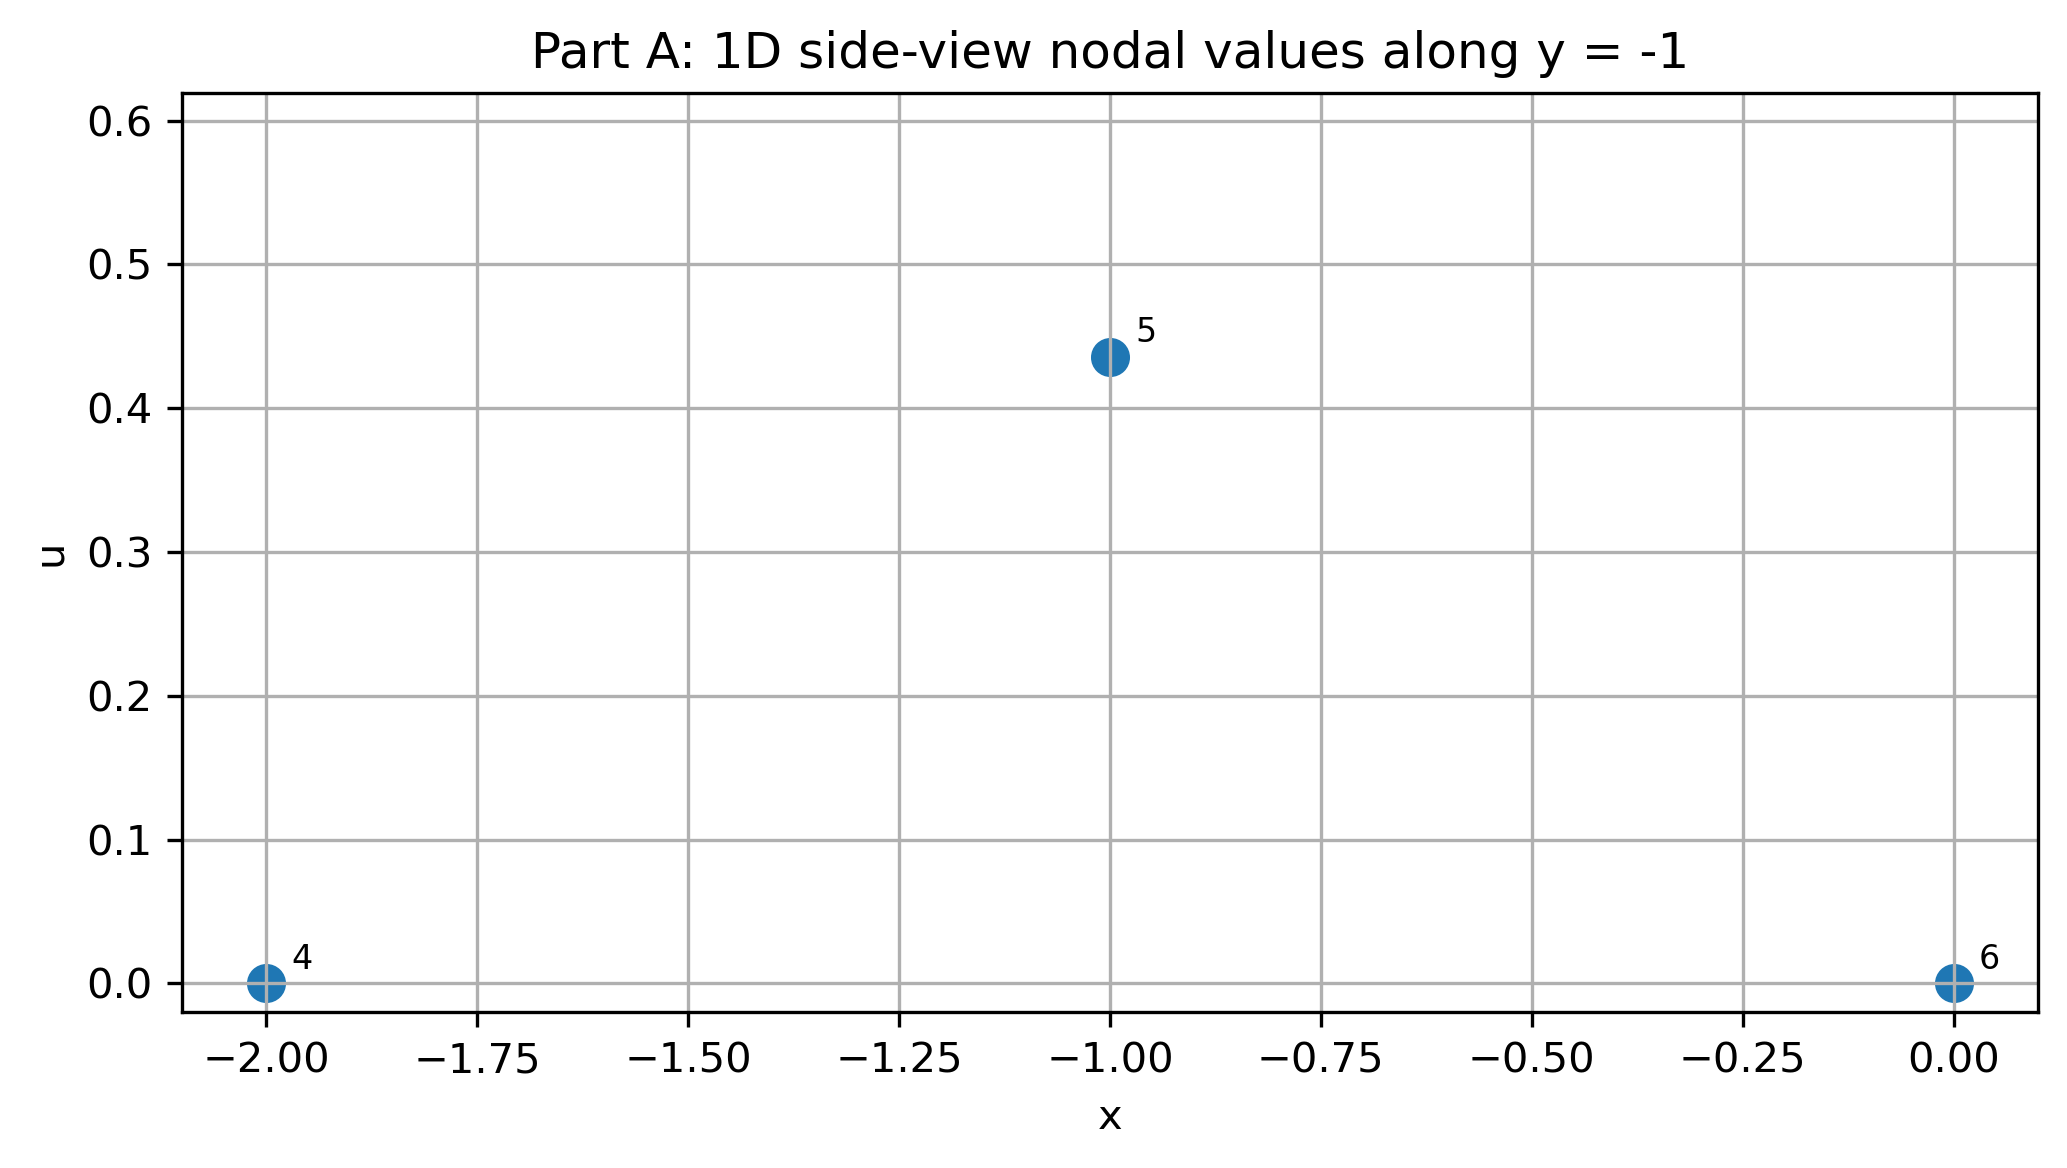
\includegraphics[width=0.80\textwidth]{images/partA_side_y_minus1.png}
\caption{Part A one-dimensional side-view nodal plot along the line $y=-1$.}
\label{fig:parta_side_y_minus1}
\end{figure}

\begin{figure}[H]
\centering
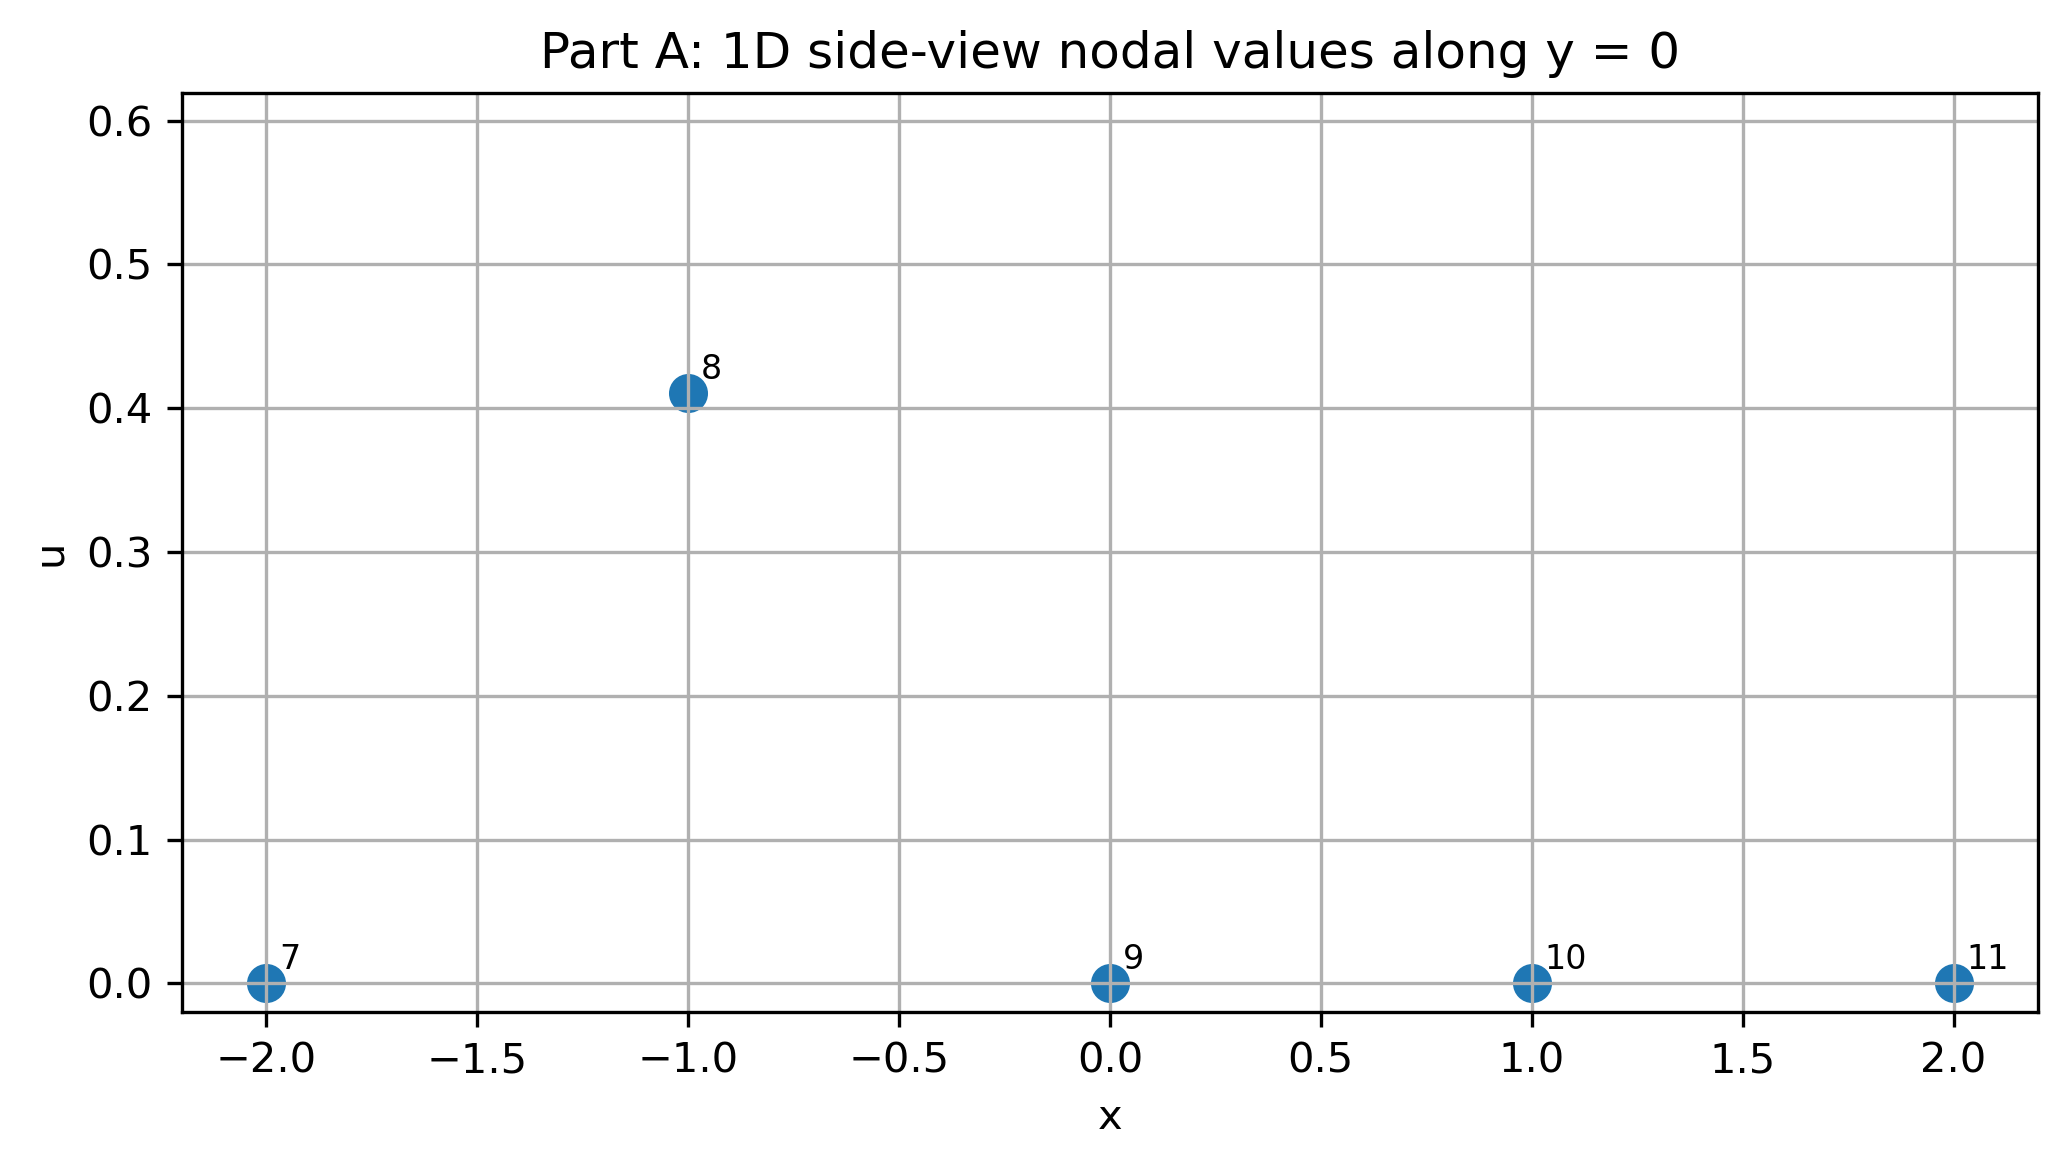
\includegraphics[width=0.80\textwidth]{images/partA_side_y_0.png}
\caption{Part A one-dimensional side-view nodal plot along the line $y=0$.}
\label{fig:parta_side_y_0}
\end{figure}

\begin{figure}[H]
\centering
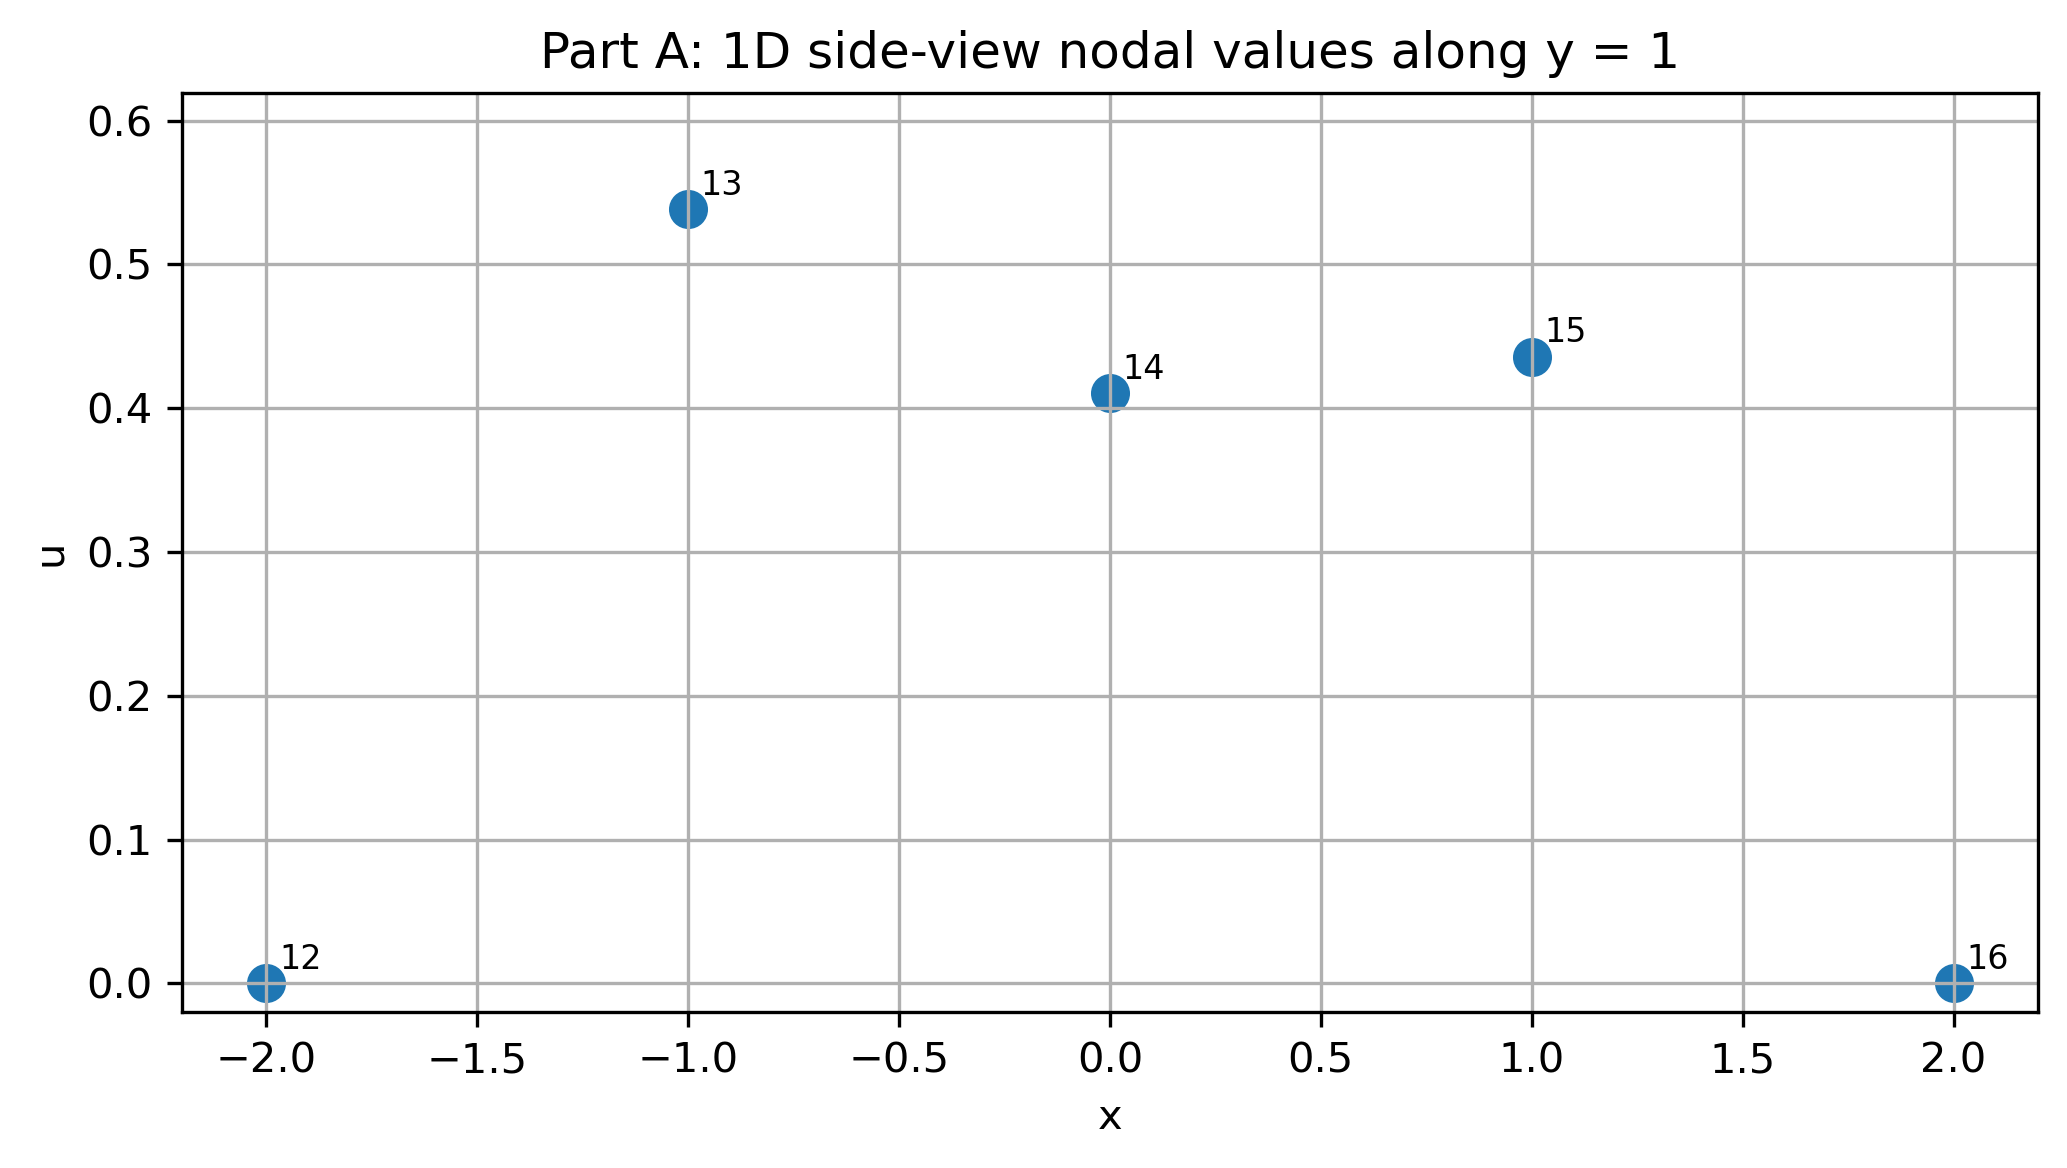
\includegraphics[width=0.80\textwidth]{images/partA_side_y_1.png}
\caption{Part A one-dimensional side-view nodal plot along the line $y=1$.}
\label{fig:parta_side_y_1}
\end{figure}

\subsection{Two-Dimensional Nodal and Contour Plots}

\begin{figure}[H]
\centering
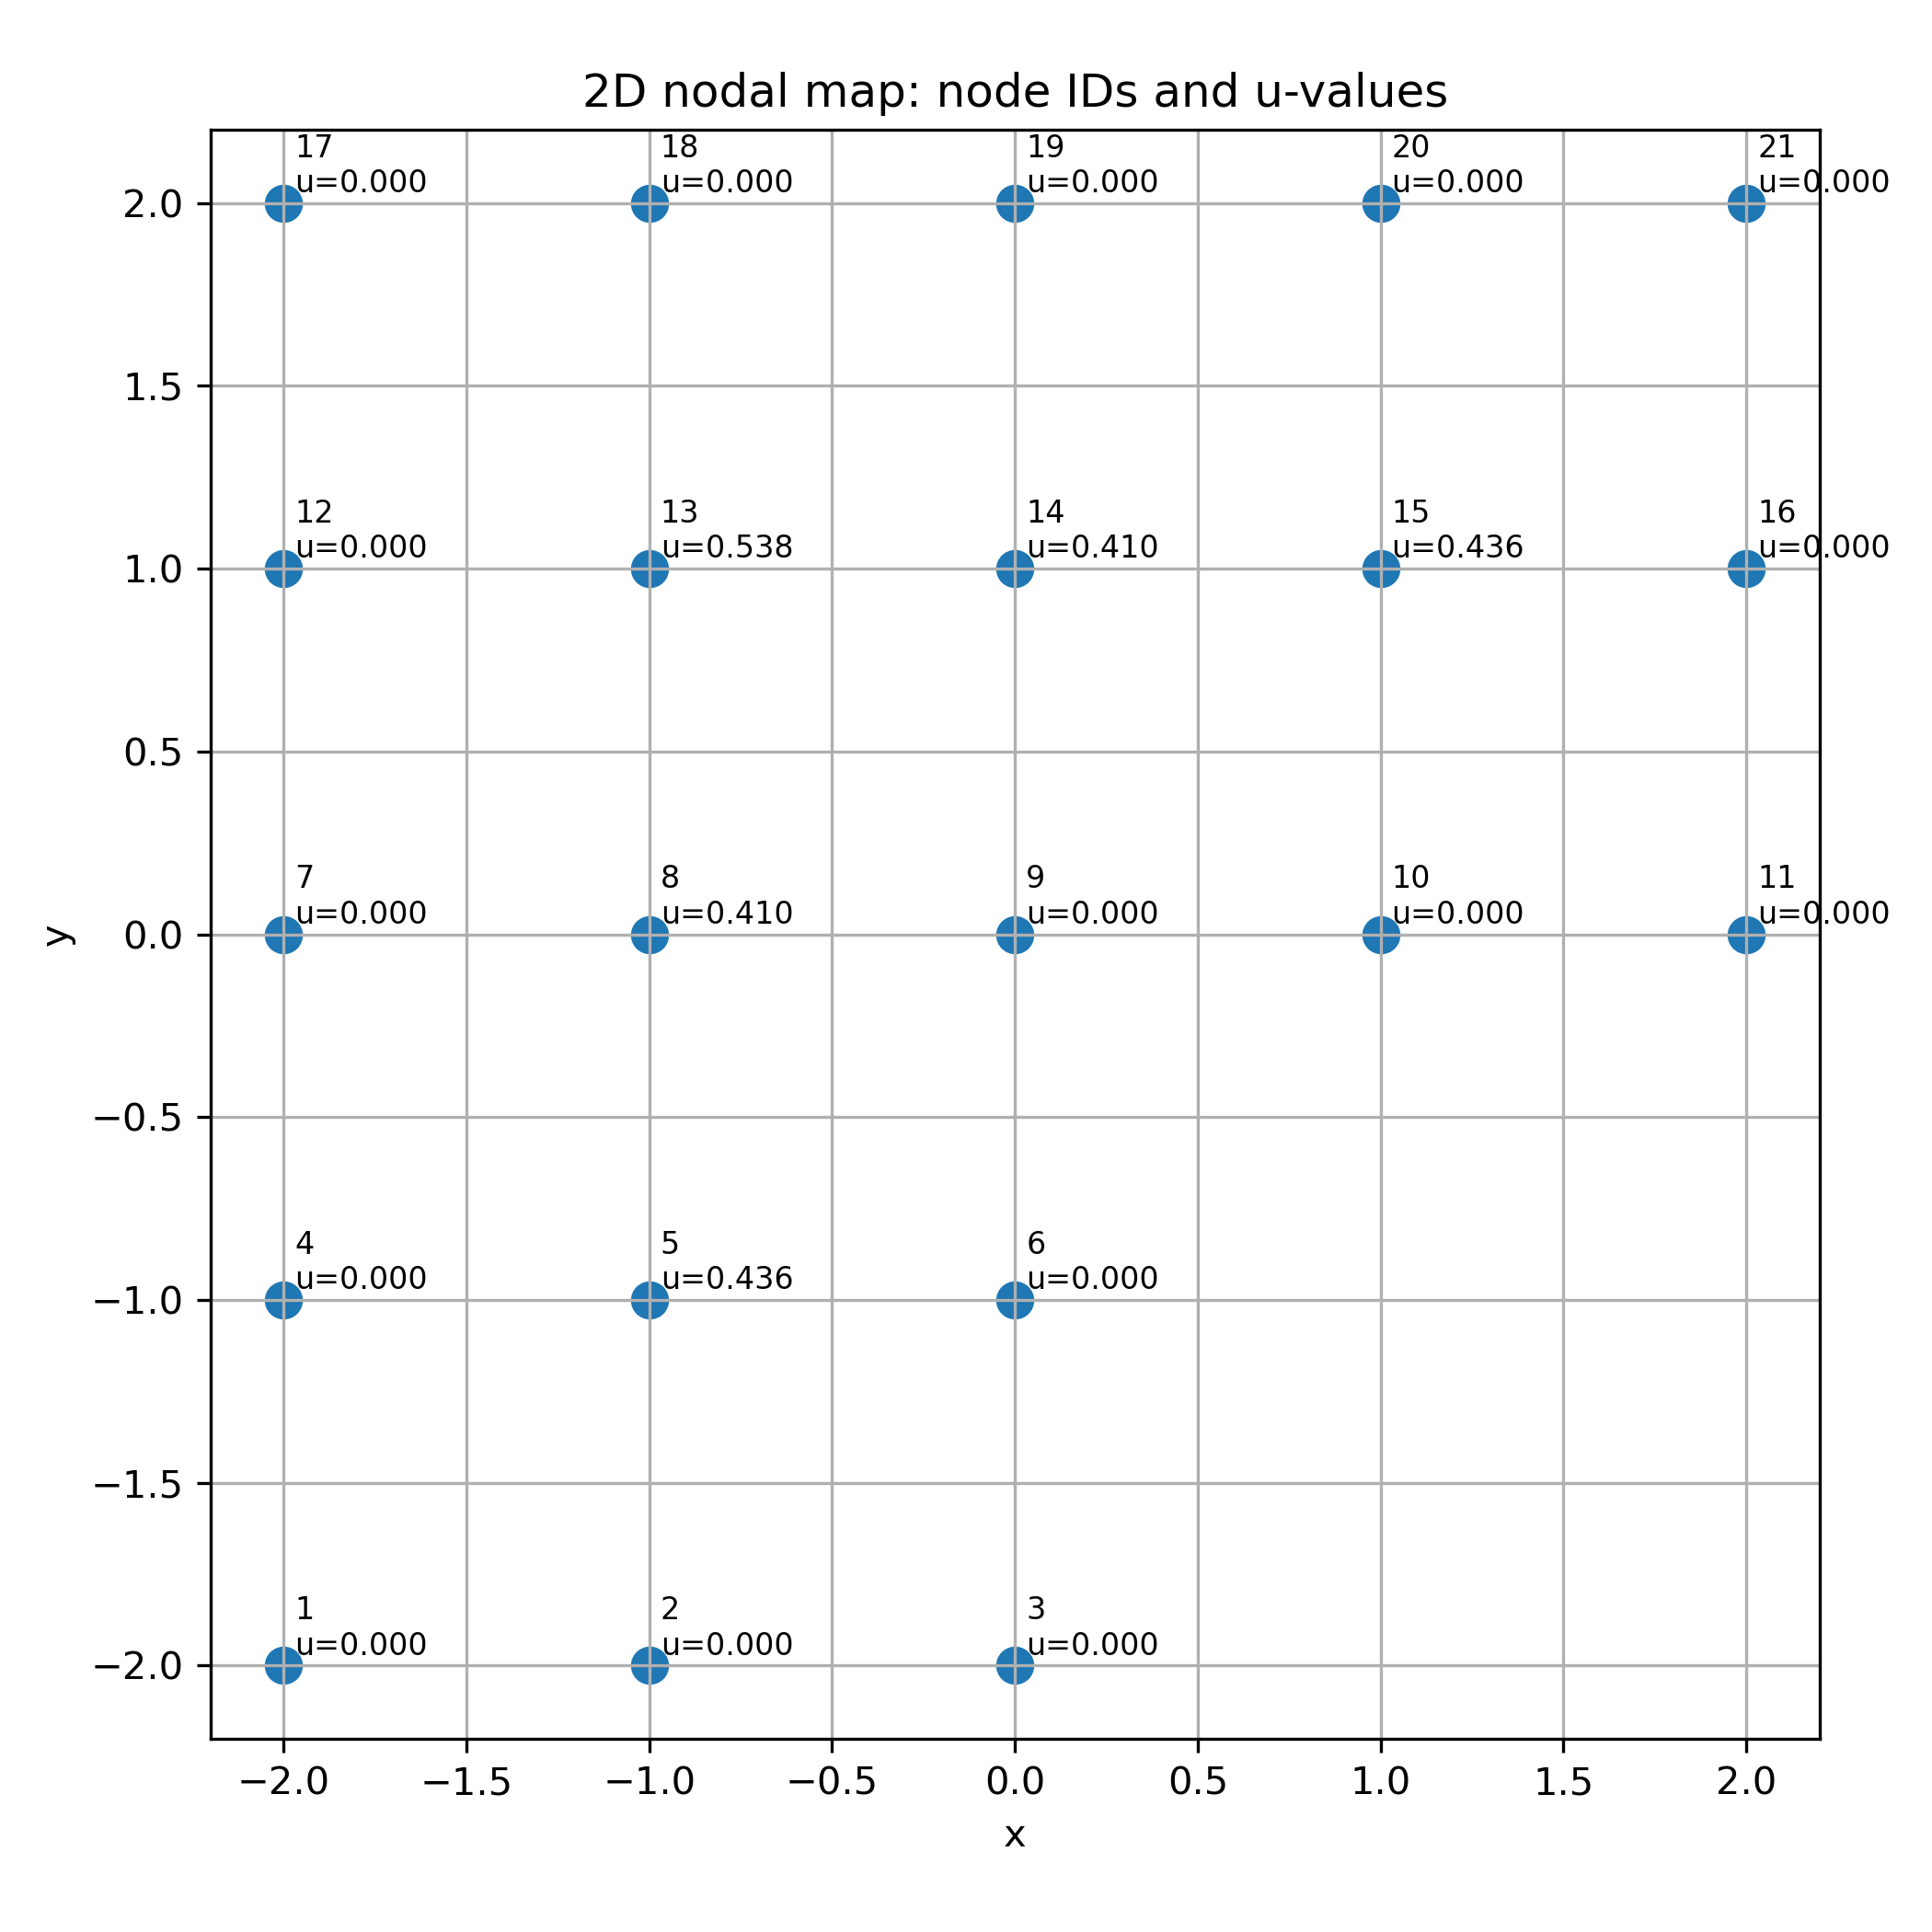
\includegraphics[width=0.80\textwidth]{images/partA_2D_nodal_map.png}
\caption{Part A two-dimensional nodal map of the computed scalar field.}
\label{fig:parta_nodal_map}
\end{figure}

\begin{figure}[H]
\centering
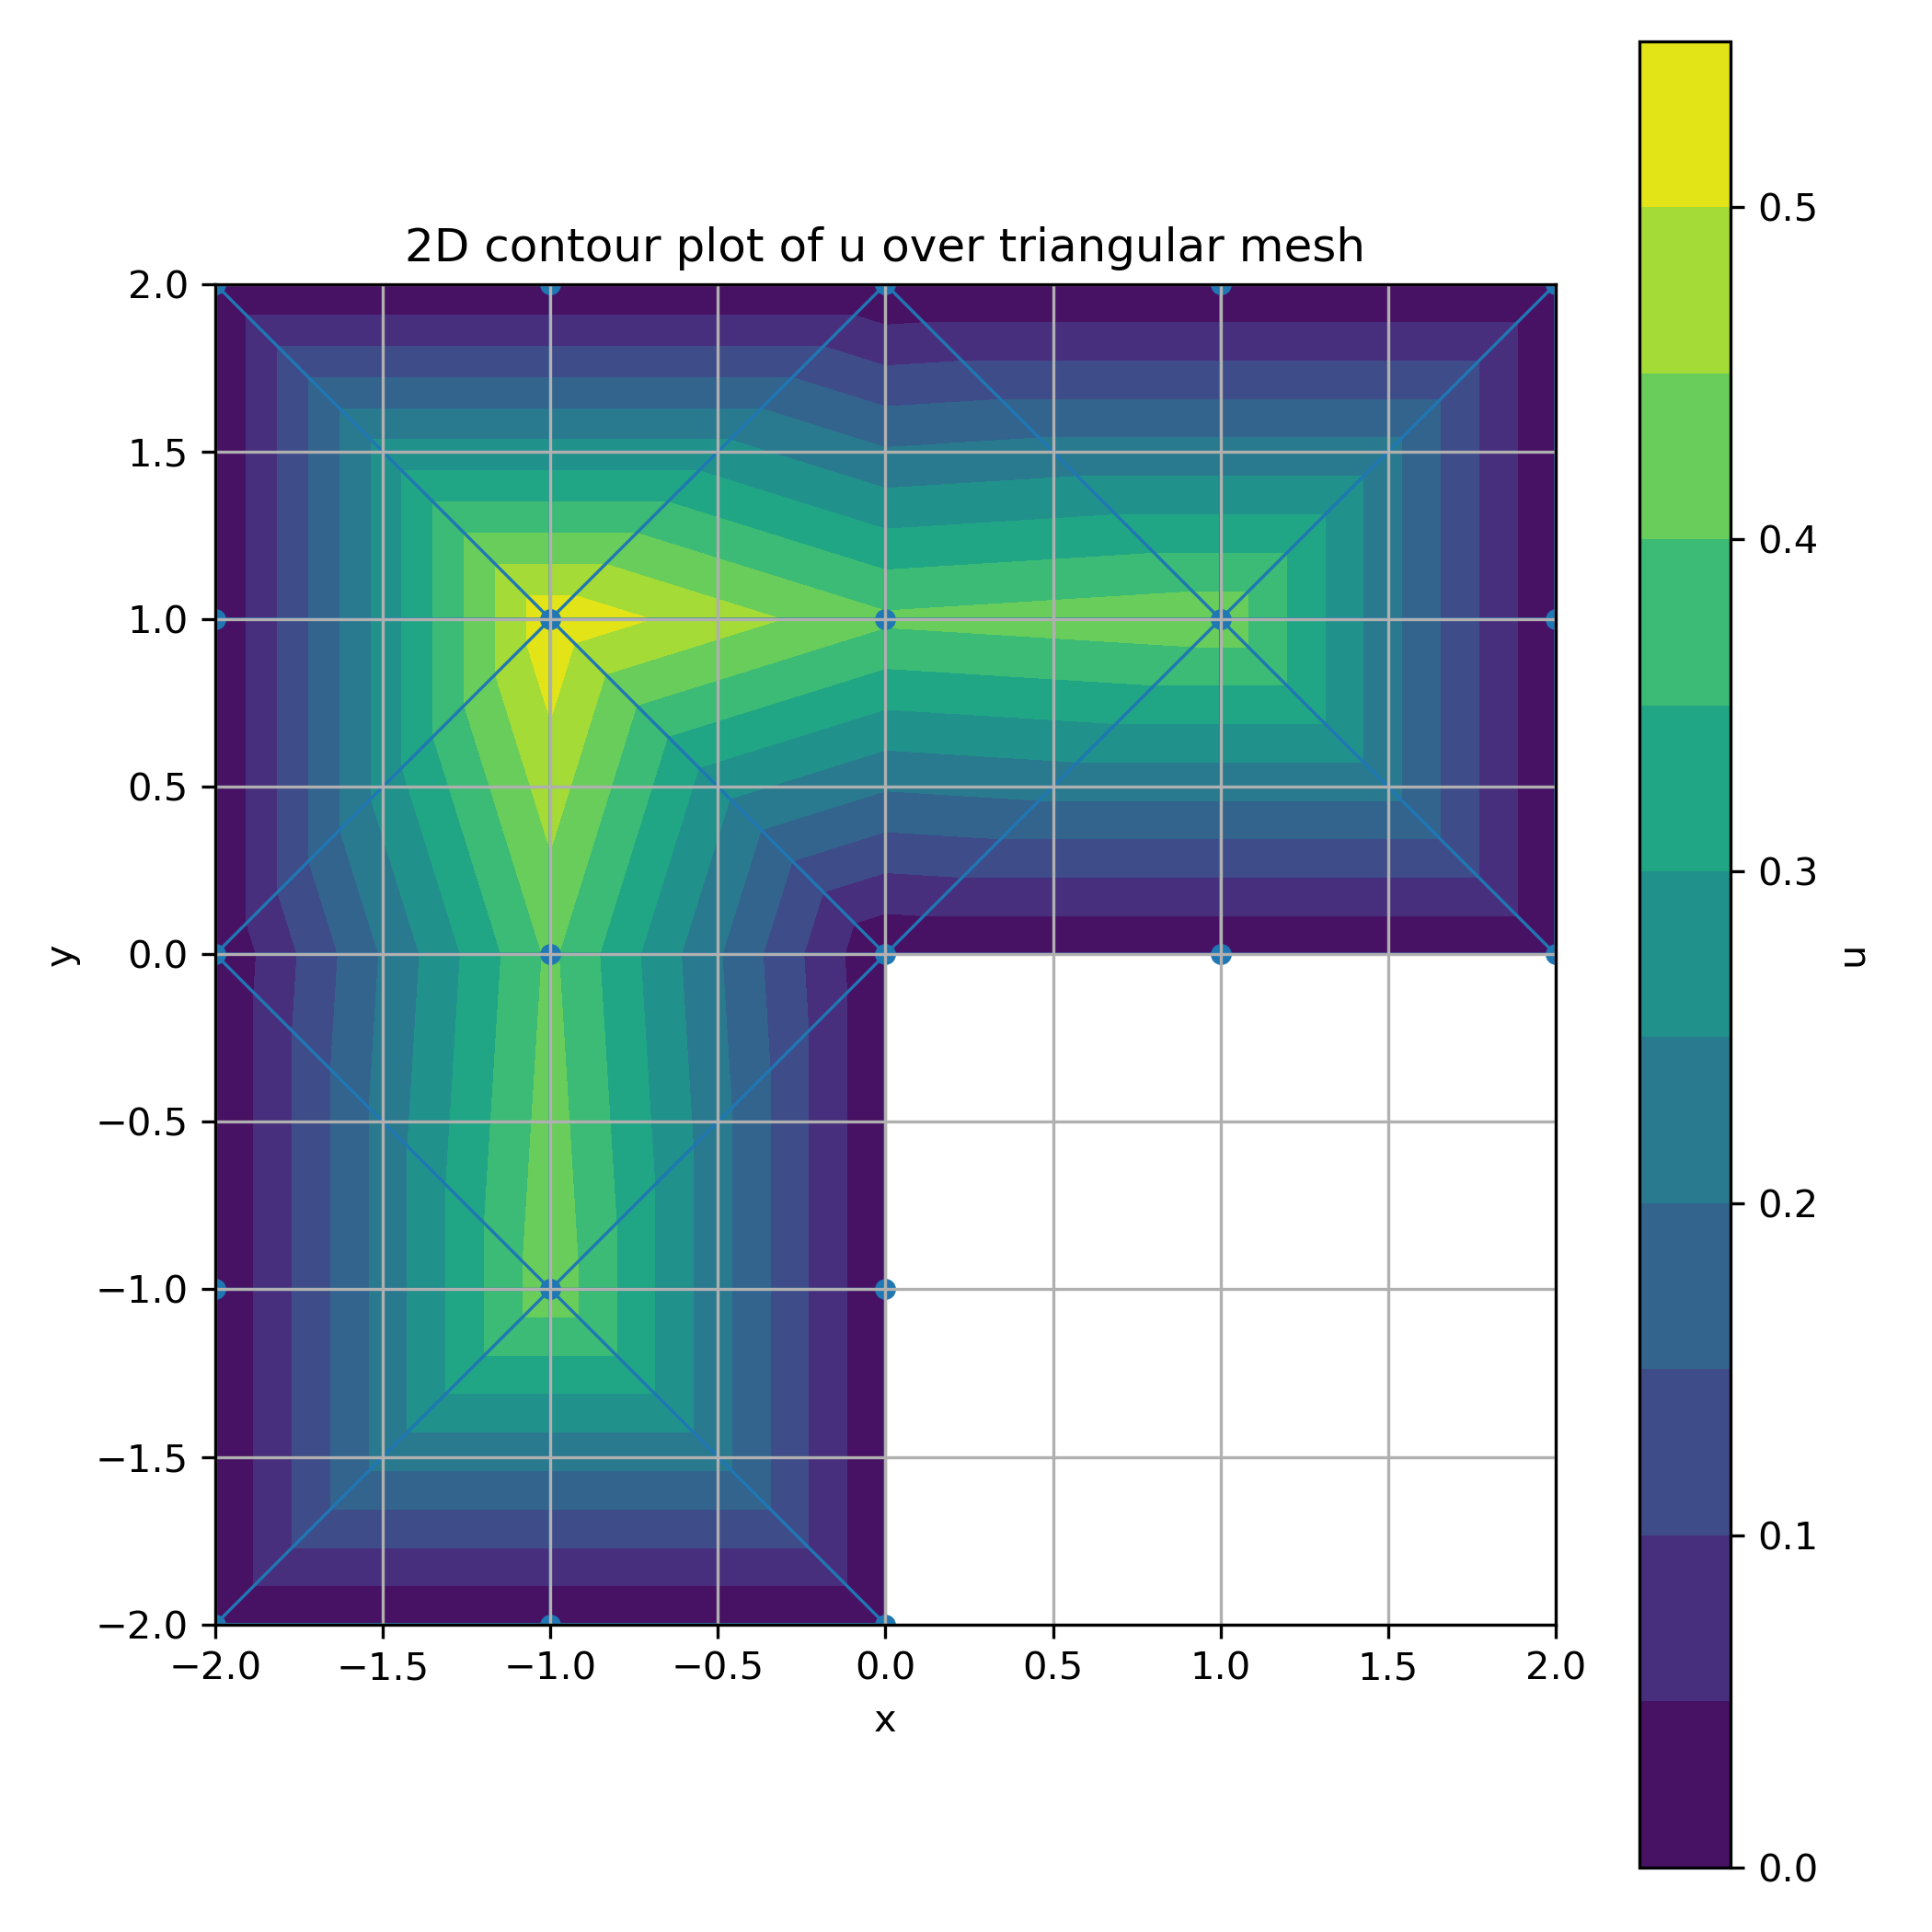
\includegraphics[width=0.80\textwidth]{images/partA_2D_contour.png}
\caption{Part A two-dimensional contour representation of the computed scalar field.}
\label{fig:parta_contour}
\end{figure}

\subsection{Three-Dimensional Nodal Plot}

\begin{figure}[H]
\centering
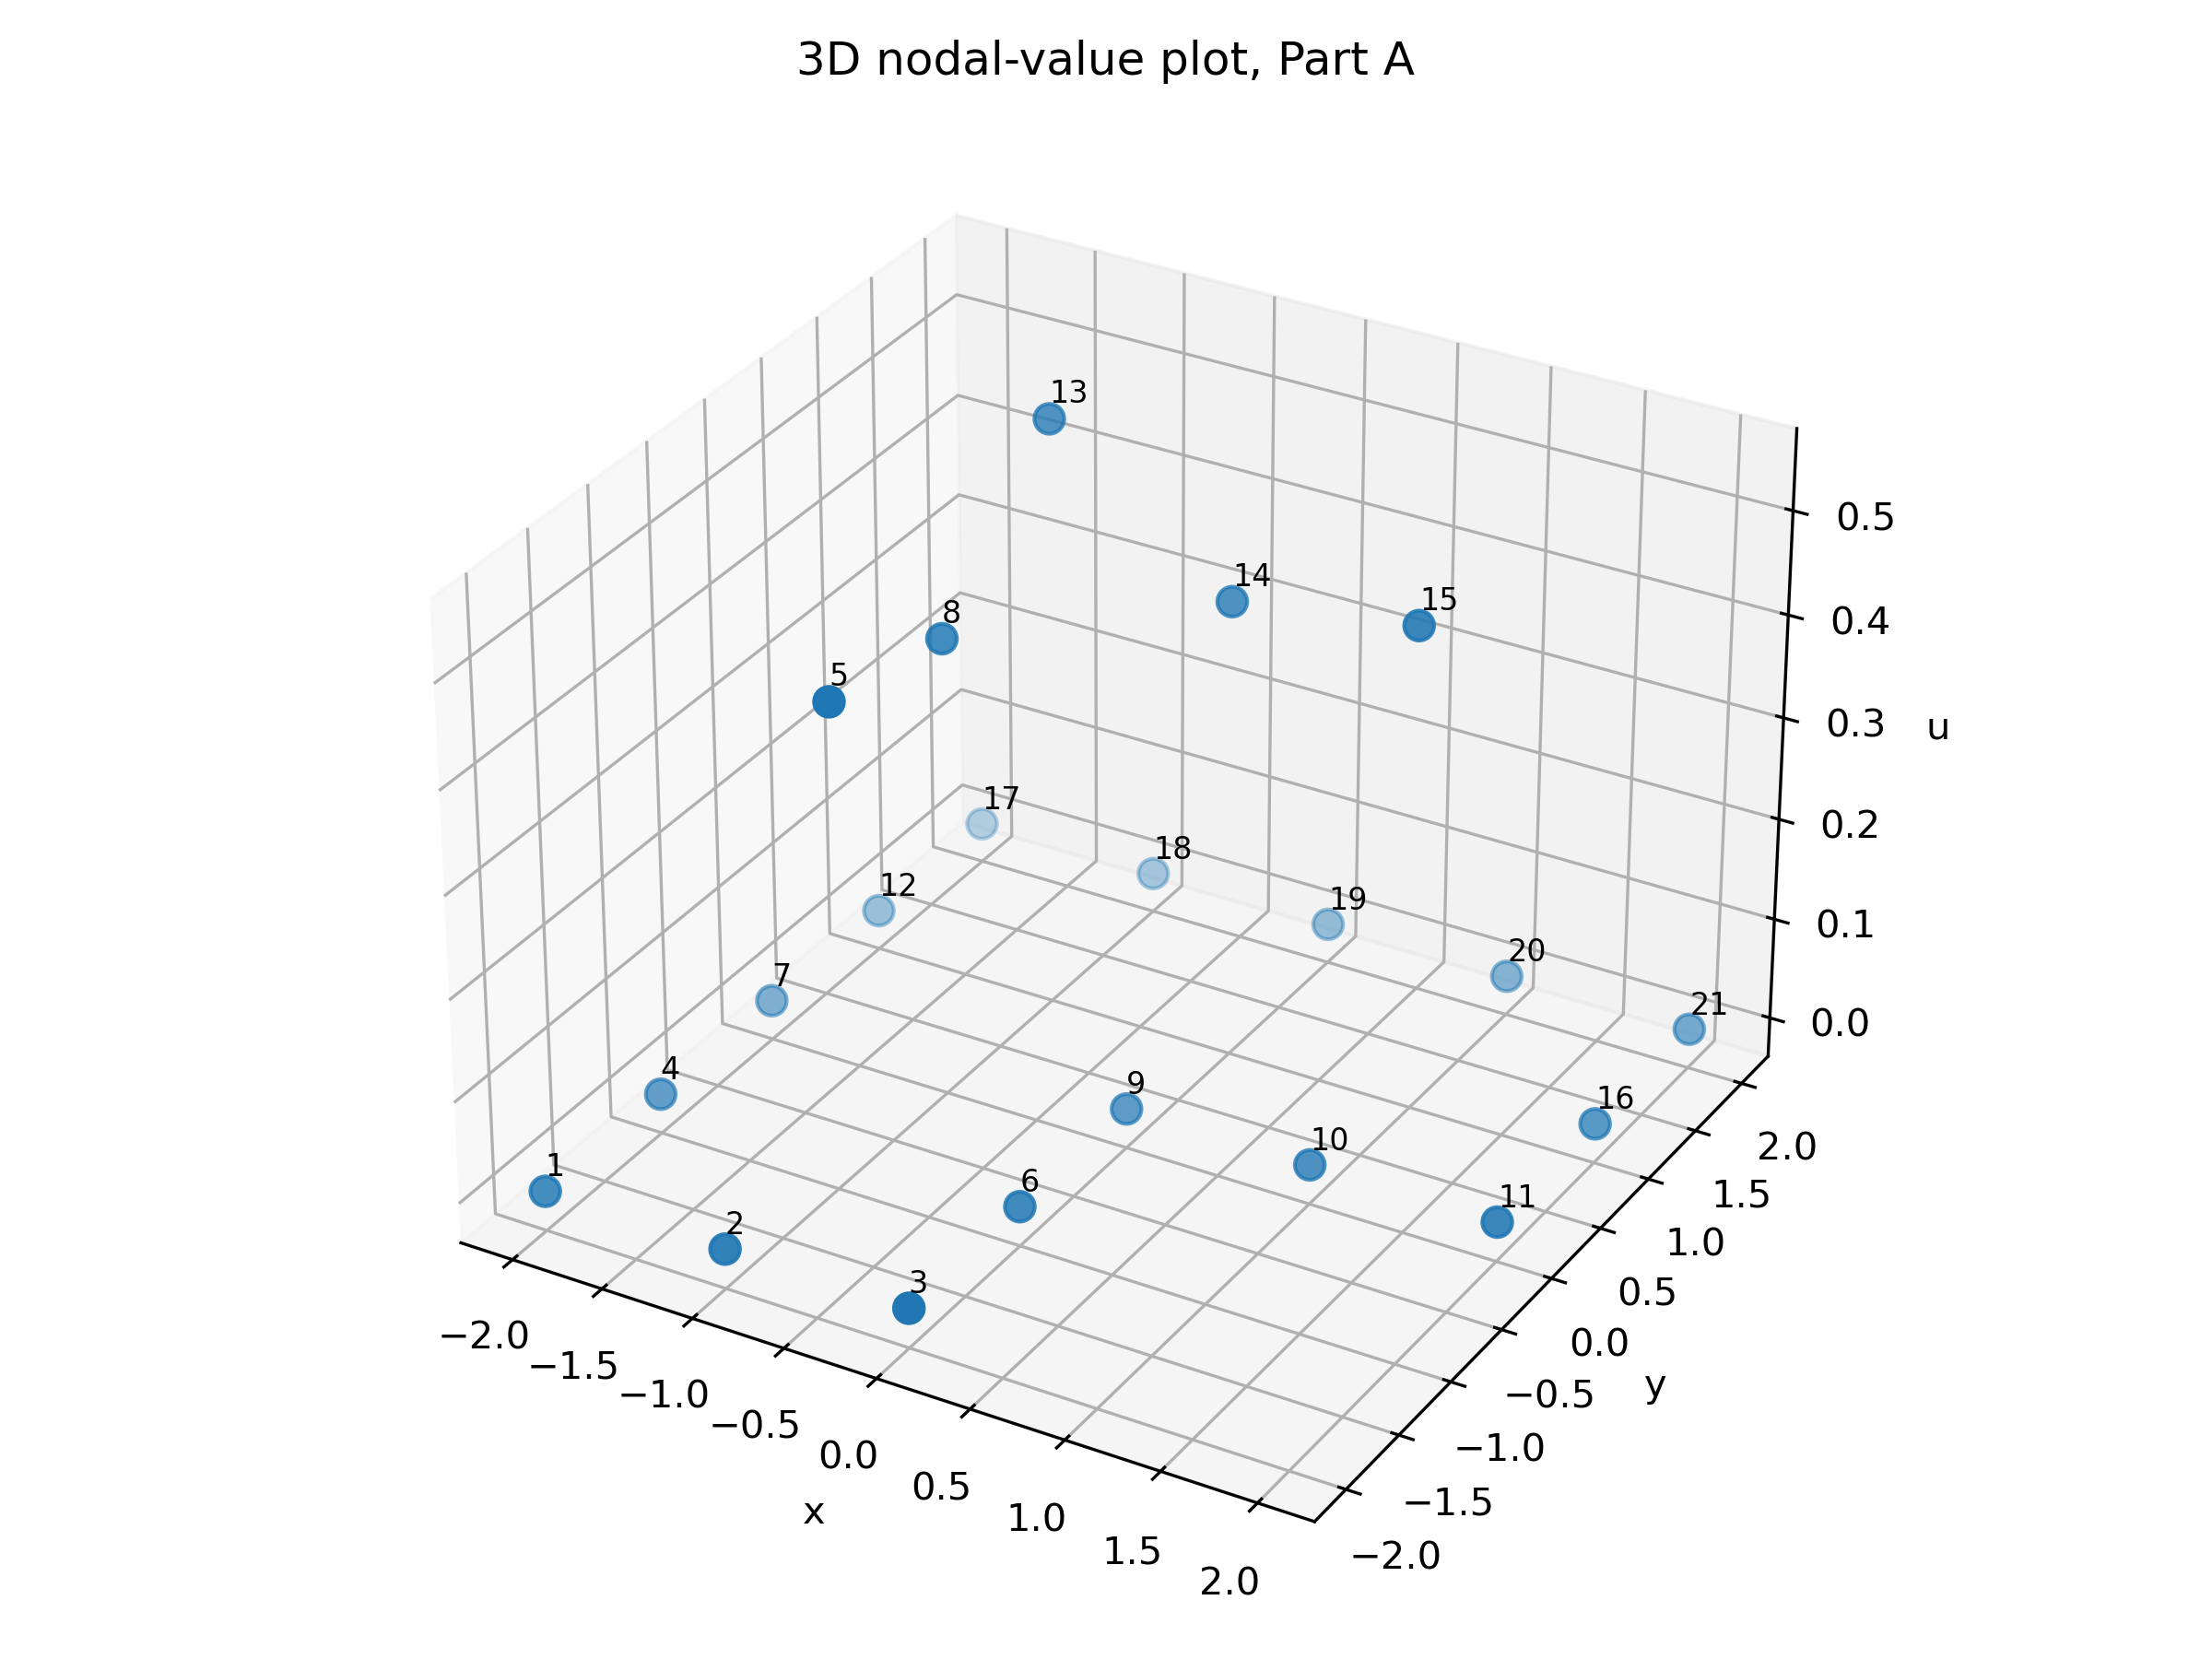
\includegraphics[width=0.80\textwidth]{images/partA_3D_points_only.png}
\caption{Part A three-dimensional nodal-value plot shown as a points-only surface.}
\label{fig:parta_3d}
\end{figure}

\subsection{Gradient Results}

For linear triangular elements,
\begin{equation}
    \grad u=\frac{1}{2A_e}
    \vect{\sum_{i=1}^3 u_i\beta_i\\\sum_{i=1}^3 u_i\gamma_i}.
\end{equation}

The gradient is constant inside each triangular element, but it can be discontinuous across element edges. Both requested points lie on element edges, so two adjacent values are reported.

At $(-0.5,0)$:
\begin{align}
    \grad u^{-} &= \vect{-0.410256\\-0.025641}
    =\vect{-16/39\\-1/39},\\
    \grad u^{+} &= \vect{-0.410256\\0.128205}
    =\vect{-16/39\\5/39},\\
    \grad u_{\mathrm{avg}} &= \vect{-0.410256\\0.051282}
    =\vect{-16/39\\2/39}.
\end{align}

At $(0,0.5)$:
\begin{align}
    \grad u^{-} &= \vect{-0.128205\\0.410256}
    =\vect{-5/39\\16/39},\\
    \grad u^{+} &= \vect{0.025641\\0.410256}
    =\vect{1/39\\16/39},\\
    \grad u_{\mathrm{avg}} &= \vect{-0.051282\\0.410256}
    =\vect{-2/39\\16/39}.
\end{align}

\subsection{Flux Results}

The requested mathematical normal flux is
\begin{equation}
    k\grad u\cdot n.
\end{equation}
For this problem, $k=1$.

On $x=2$, the outward normal is
\begin{equation}
    n=\vect{1\\0}.
\end{equation}
Thus,
\begin{equation}
    k\grad u\cdot n=-0.435897=-\frac{17}{39}.
\end{equation}

On $y=-2$, the outward normal is
\begin{equation}
    n=\vect{0\\-1}.
\end{equation}
Thus,
\begin{equation}
    k\grad u\cdot n=-0.435897=-\frac{17}{39}.
\end{equation}

\section{Part B: Bilinear Rectangular Elements}

\subsection{Reduced System}

The reduced stiffness matrix is
\begin{equation}
K_{ff}^{\square}=\mat{
8/3 & -1/3 & 0 & 0 & 0\\
-1/3 & 8/3 & -1/3 & -1/3 & 0\\
0 & -1/3 & 8/3 & -1/3 & 0\\
0 & -1/3 & -1/3 & 8/3 & -1/3\\
0 & 0 & 0 & -1/3 & 8/3
}.
\end{equation}

The reduced force vector is
\begin{equation}
F_f^{\square}=\vect{1\\1\\1\\1\\1}.
\end{equation}

Thus,
\begin{equation}
K_{ff}^{\square}U_f^{\square}=F_f^{\square}.
\end{equation}

\subsection{Nodal Solution}

Solving gives
\begin{equation}
U_f^{\square}=\vect{
0.445755\\
0.566038\\
0.516509\\
0.566038\\
0.445755
}
=
\vect{
189/424\\
30/53\\
219/424\\
30/53\\
189/424
}.
\end{equation}

\begin{table}[H]
\centering
\caption{Part B nodal solution using bilinear rectangular elements.}
\begin{tabular}{rrrr}
\toprule
Node & $x$ & $y$ & $u$ \\
\midrule
1  & -2 & -2 & 0.000000 \\
2  & -1 & -2 & 0.000000 \\
3  &  0 & -2 & 0.000000 \\
4  & -2 & -1 & 0.000000 \\
5  & -1 & -1 & 0.445755 \\
6  &  0 & -1 & 0.000000 \\
7  & -2 &  0 & 0.000000 \\
8  & -1 &  0 & 0.566038 \\
9  &  0 &  0 & 0.000000 \\
10 &  1 &  0 & 0.000000 \\
11 &  2 &  0 & 0.000000 \\
12 & -2 &  1 & 0.000000 \\
13 & -1 &  1 & 0.516509 \\
14 &  0 &  1 & 0.566038 \\
15 &  1 &  1 & 0.445755 \\
16 &  2 &  1 & 0.000000 \\
17 & -2 &  2 & 0.000000 \\
18 & -1 &  2 & 0.000000 \\
19 &  0 &  2 & 0.000000 \\
20 &  1 &  2 & 0.000000 \\
21 &  2 &  2 & 0.000000 \\
\bottomrule
\end{tabular}
\end{table}

The maximum value is
\begin{equation}
    u_{\max}^{\square}=u_8=u_{14}=0.566038.
\end{equation}

\subsection{One-Dimensional Side-View Plots}

\begin{figure}[H]
\centering
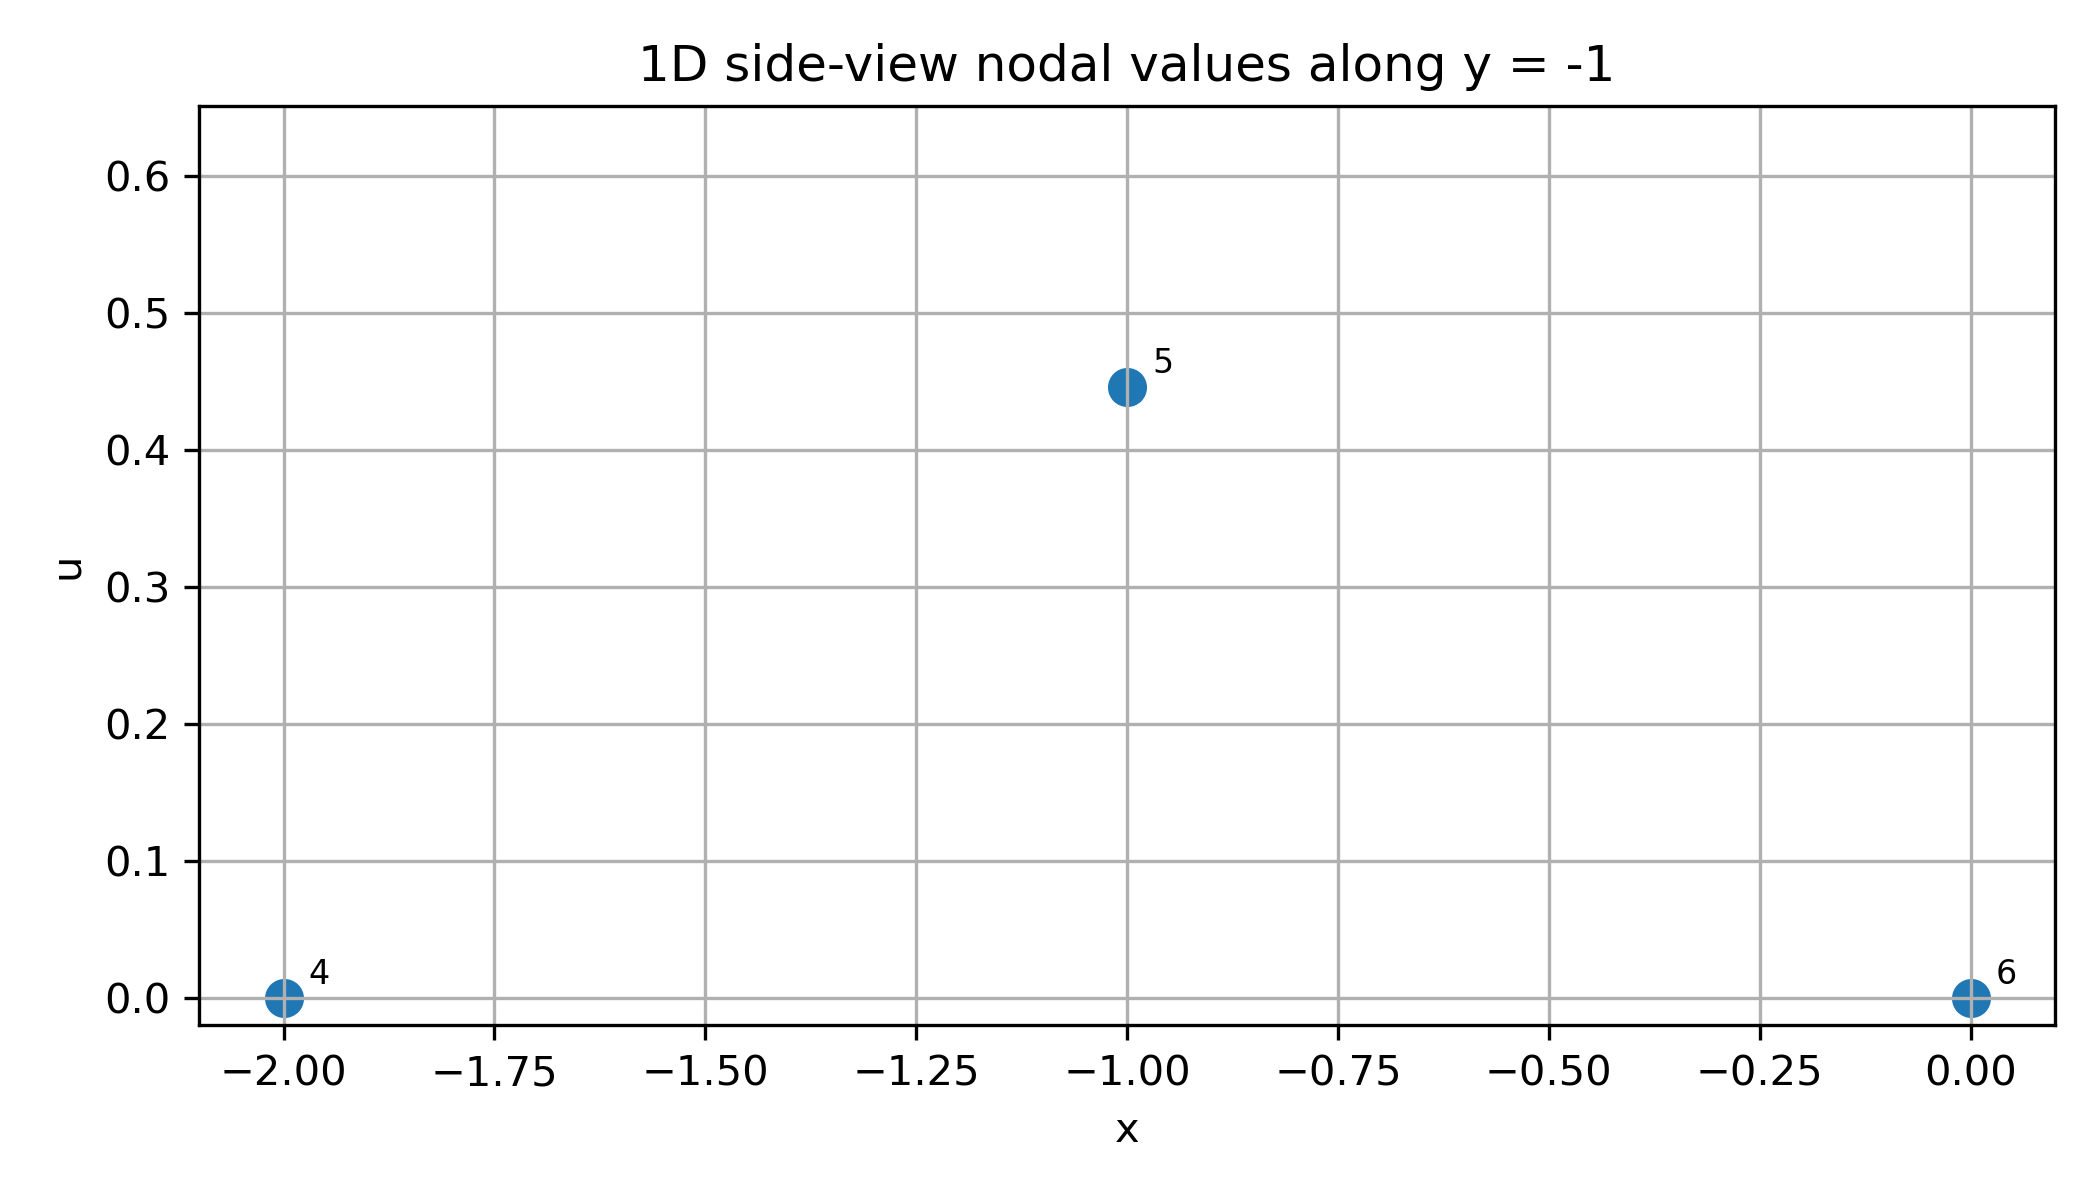
\includegraphics[width=0.80\textwidth]{images/partB_side_y_minus1.png}
\caption{Part B one-dimensional side-view nodal plot along the line $y=-1$.}
\label{fig:partb_side_y_minus1}
\end{figure}

\begin{figure}[H]
\centering
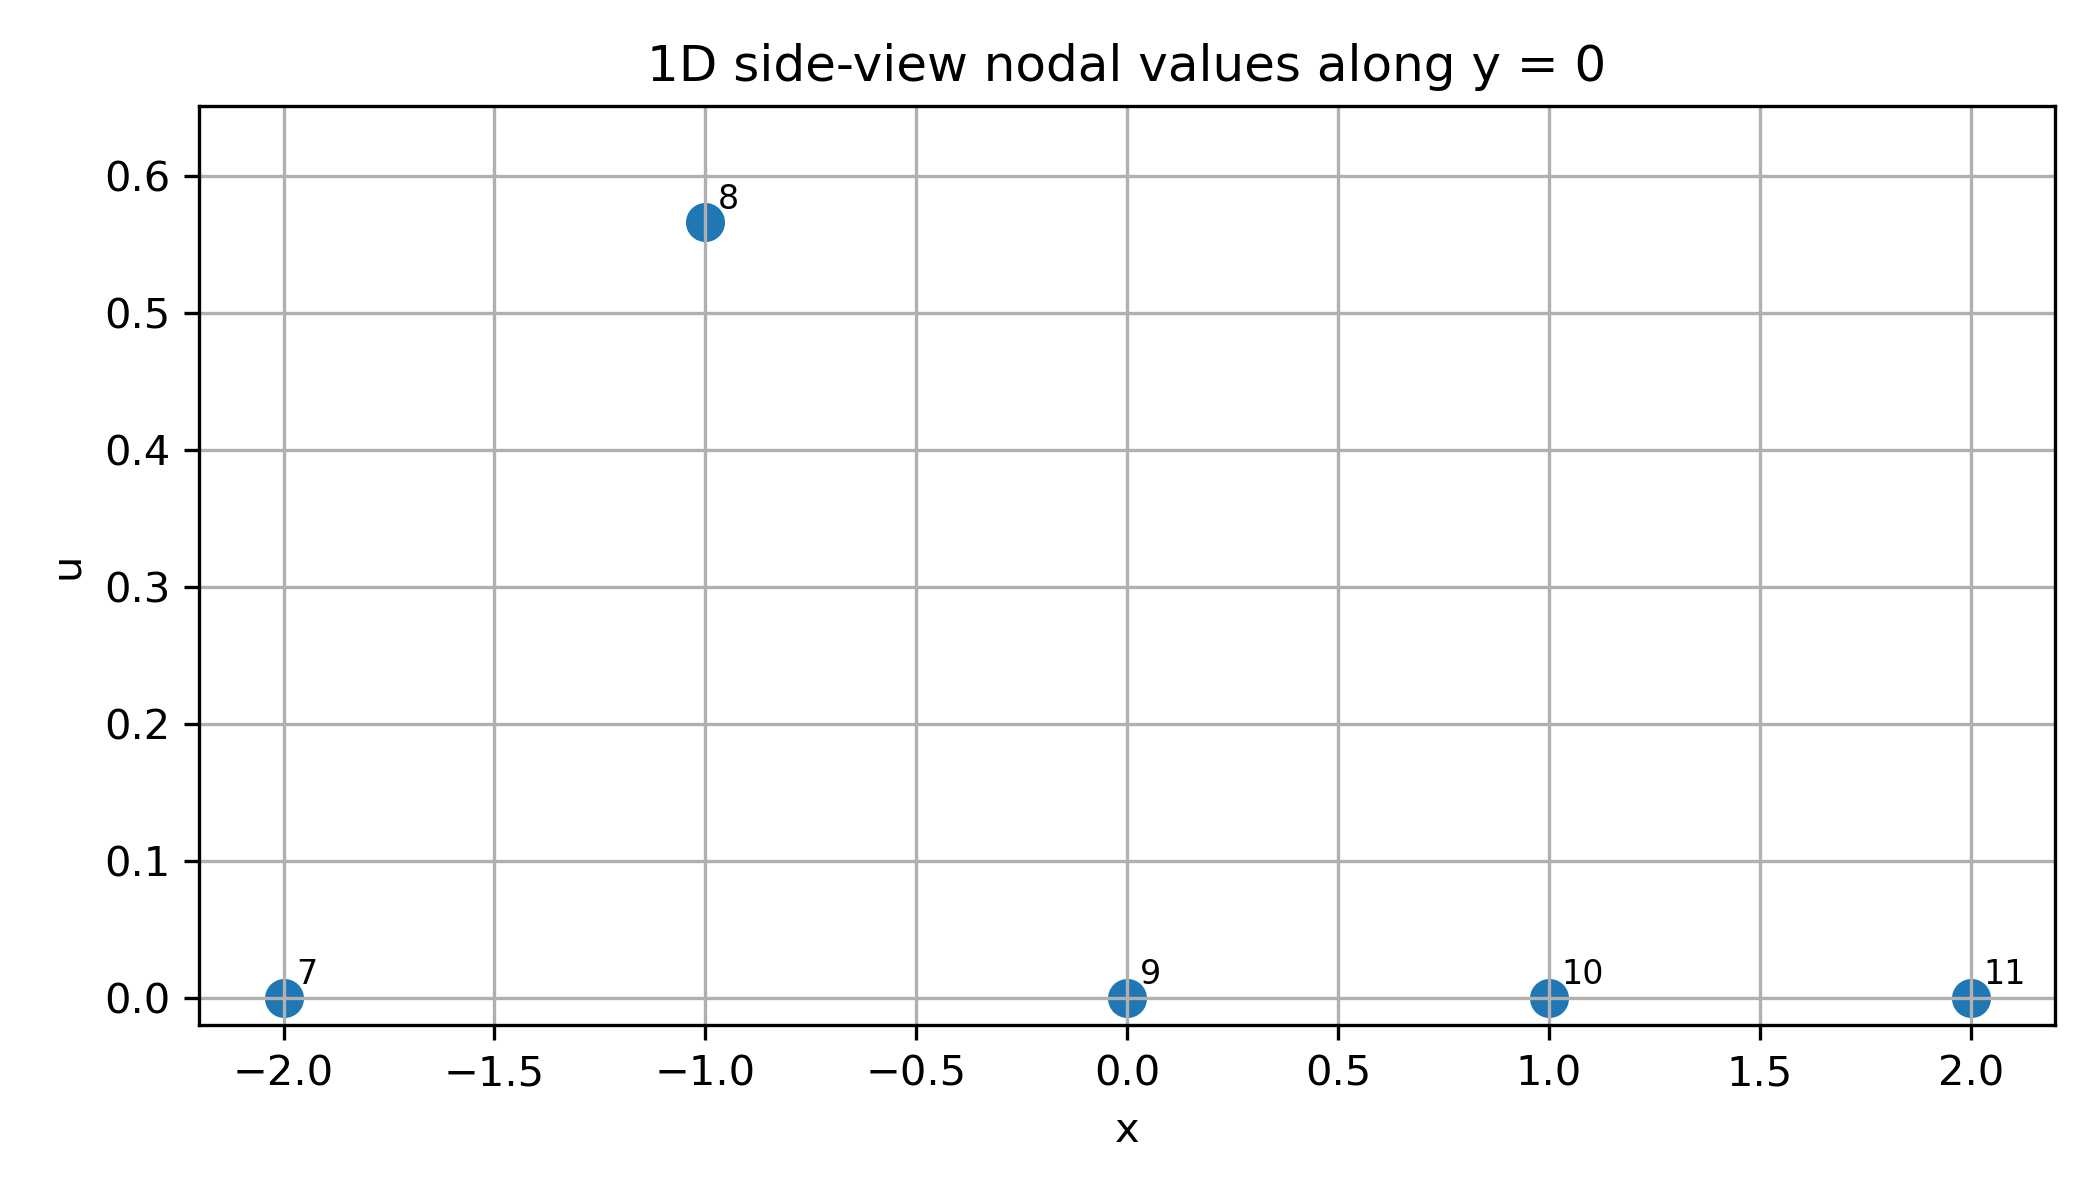
\includegraphics[width=0.80\textwidth]{images/partB_side_y_0.png}
\caption{Part B one-dimensional side-view nodal plot along the line $y=0$.}
\label{fig:partb_side_y_0}
\end{figure}

\begin{figure}[H]
\centering
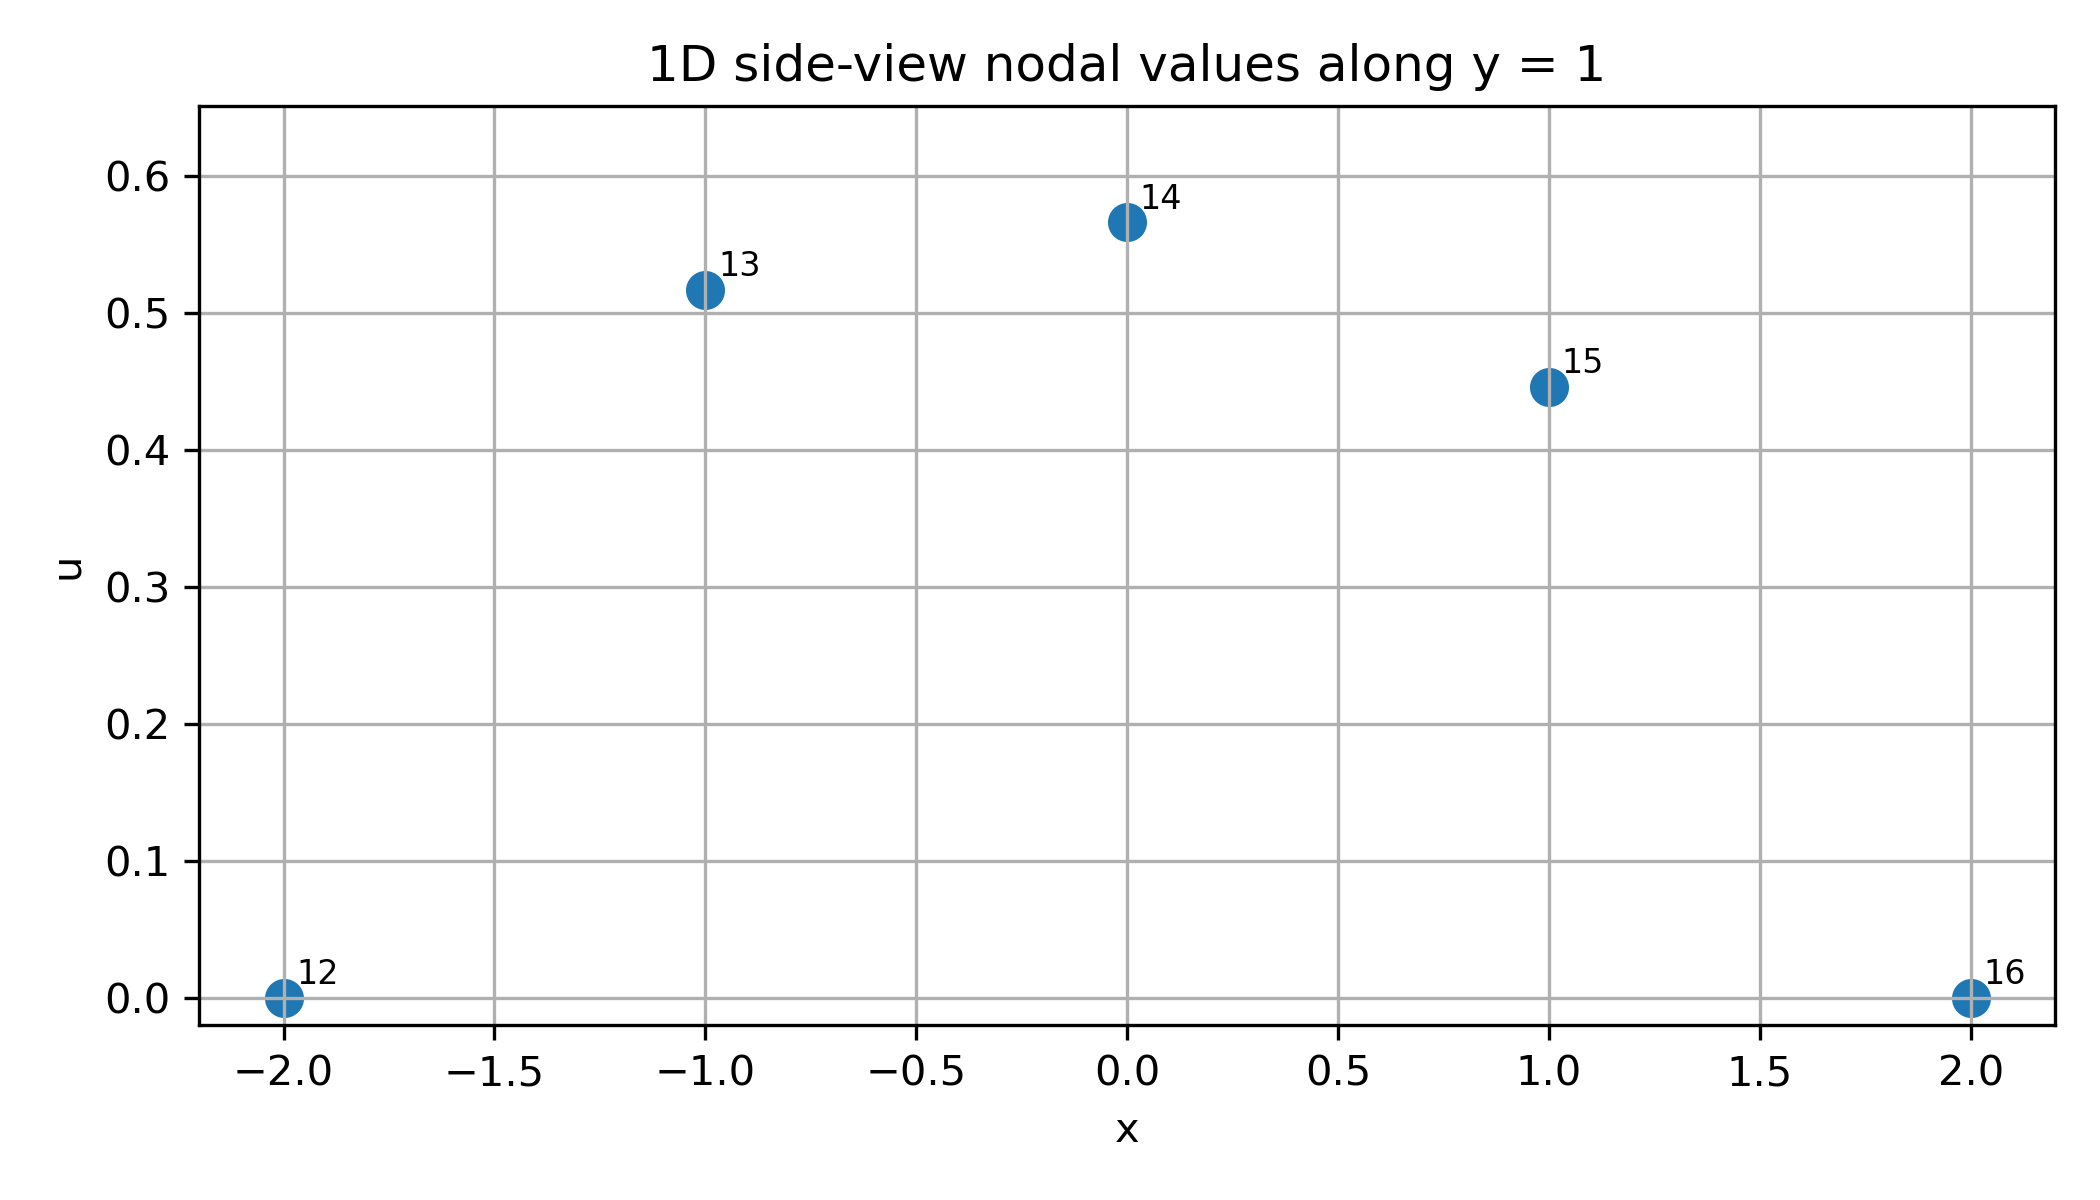
\includegraphics[width=0.80\textwidth]{images/partB_side_y_1.png}
\caption{Part B one-dimensional side-view nodal plot along the line $y=1$.}
\label{fig:partb_side_y_1}
\end{figure}

\subsection{Two-Dimensional Nodal and Cell-Average Plots}

\begin{figure}[H]
\centering
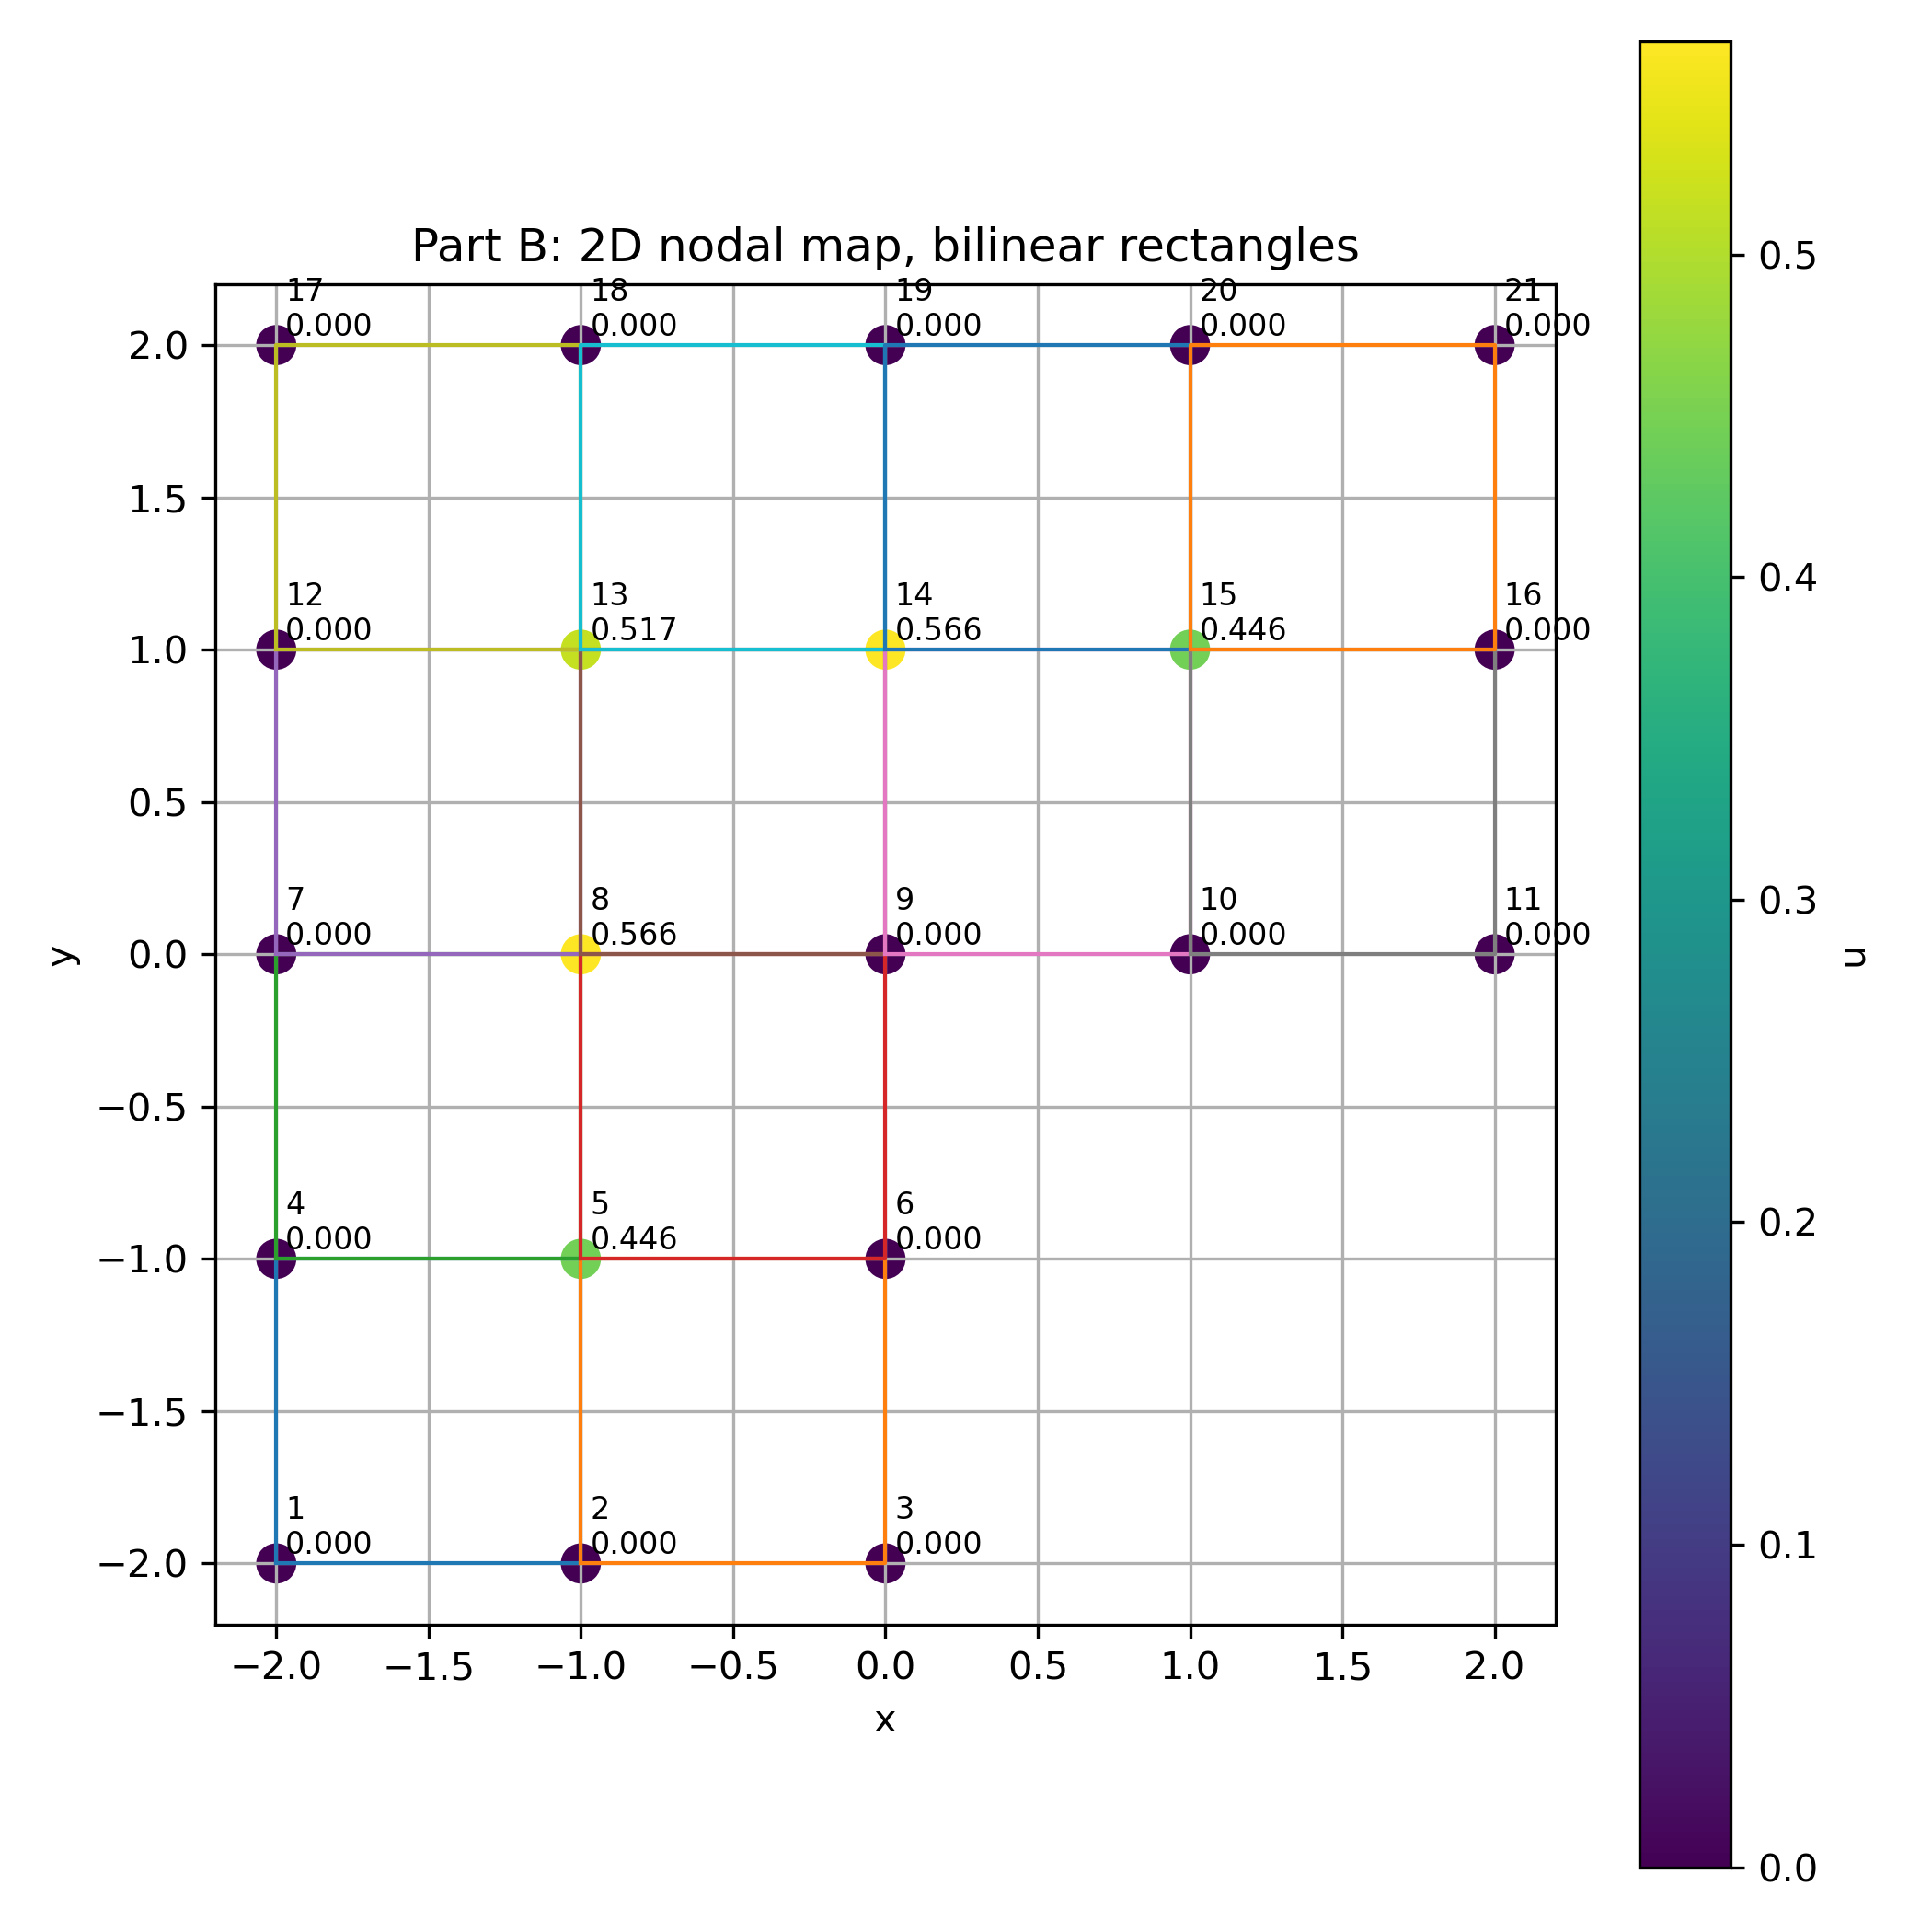
\includegraphics[width=0.80\textwidth]{images/partB_2D_nodal_map.png}
\caption{Part B two-dimensional nodal map of the computed scalar field.}
\label{fig:partb_nodal_map}
\end{figure}

\begin{figure}[H]
\centering
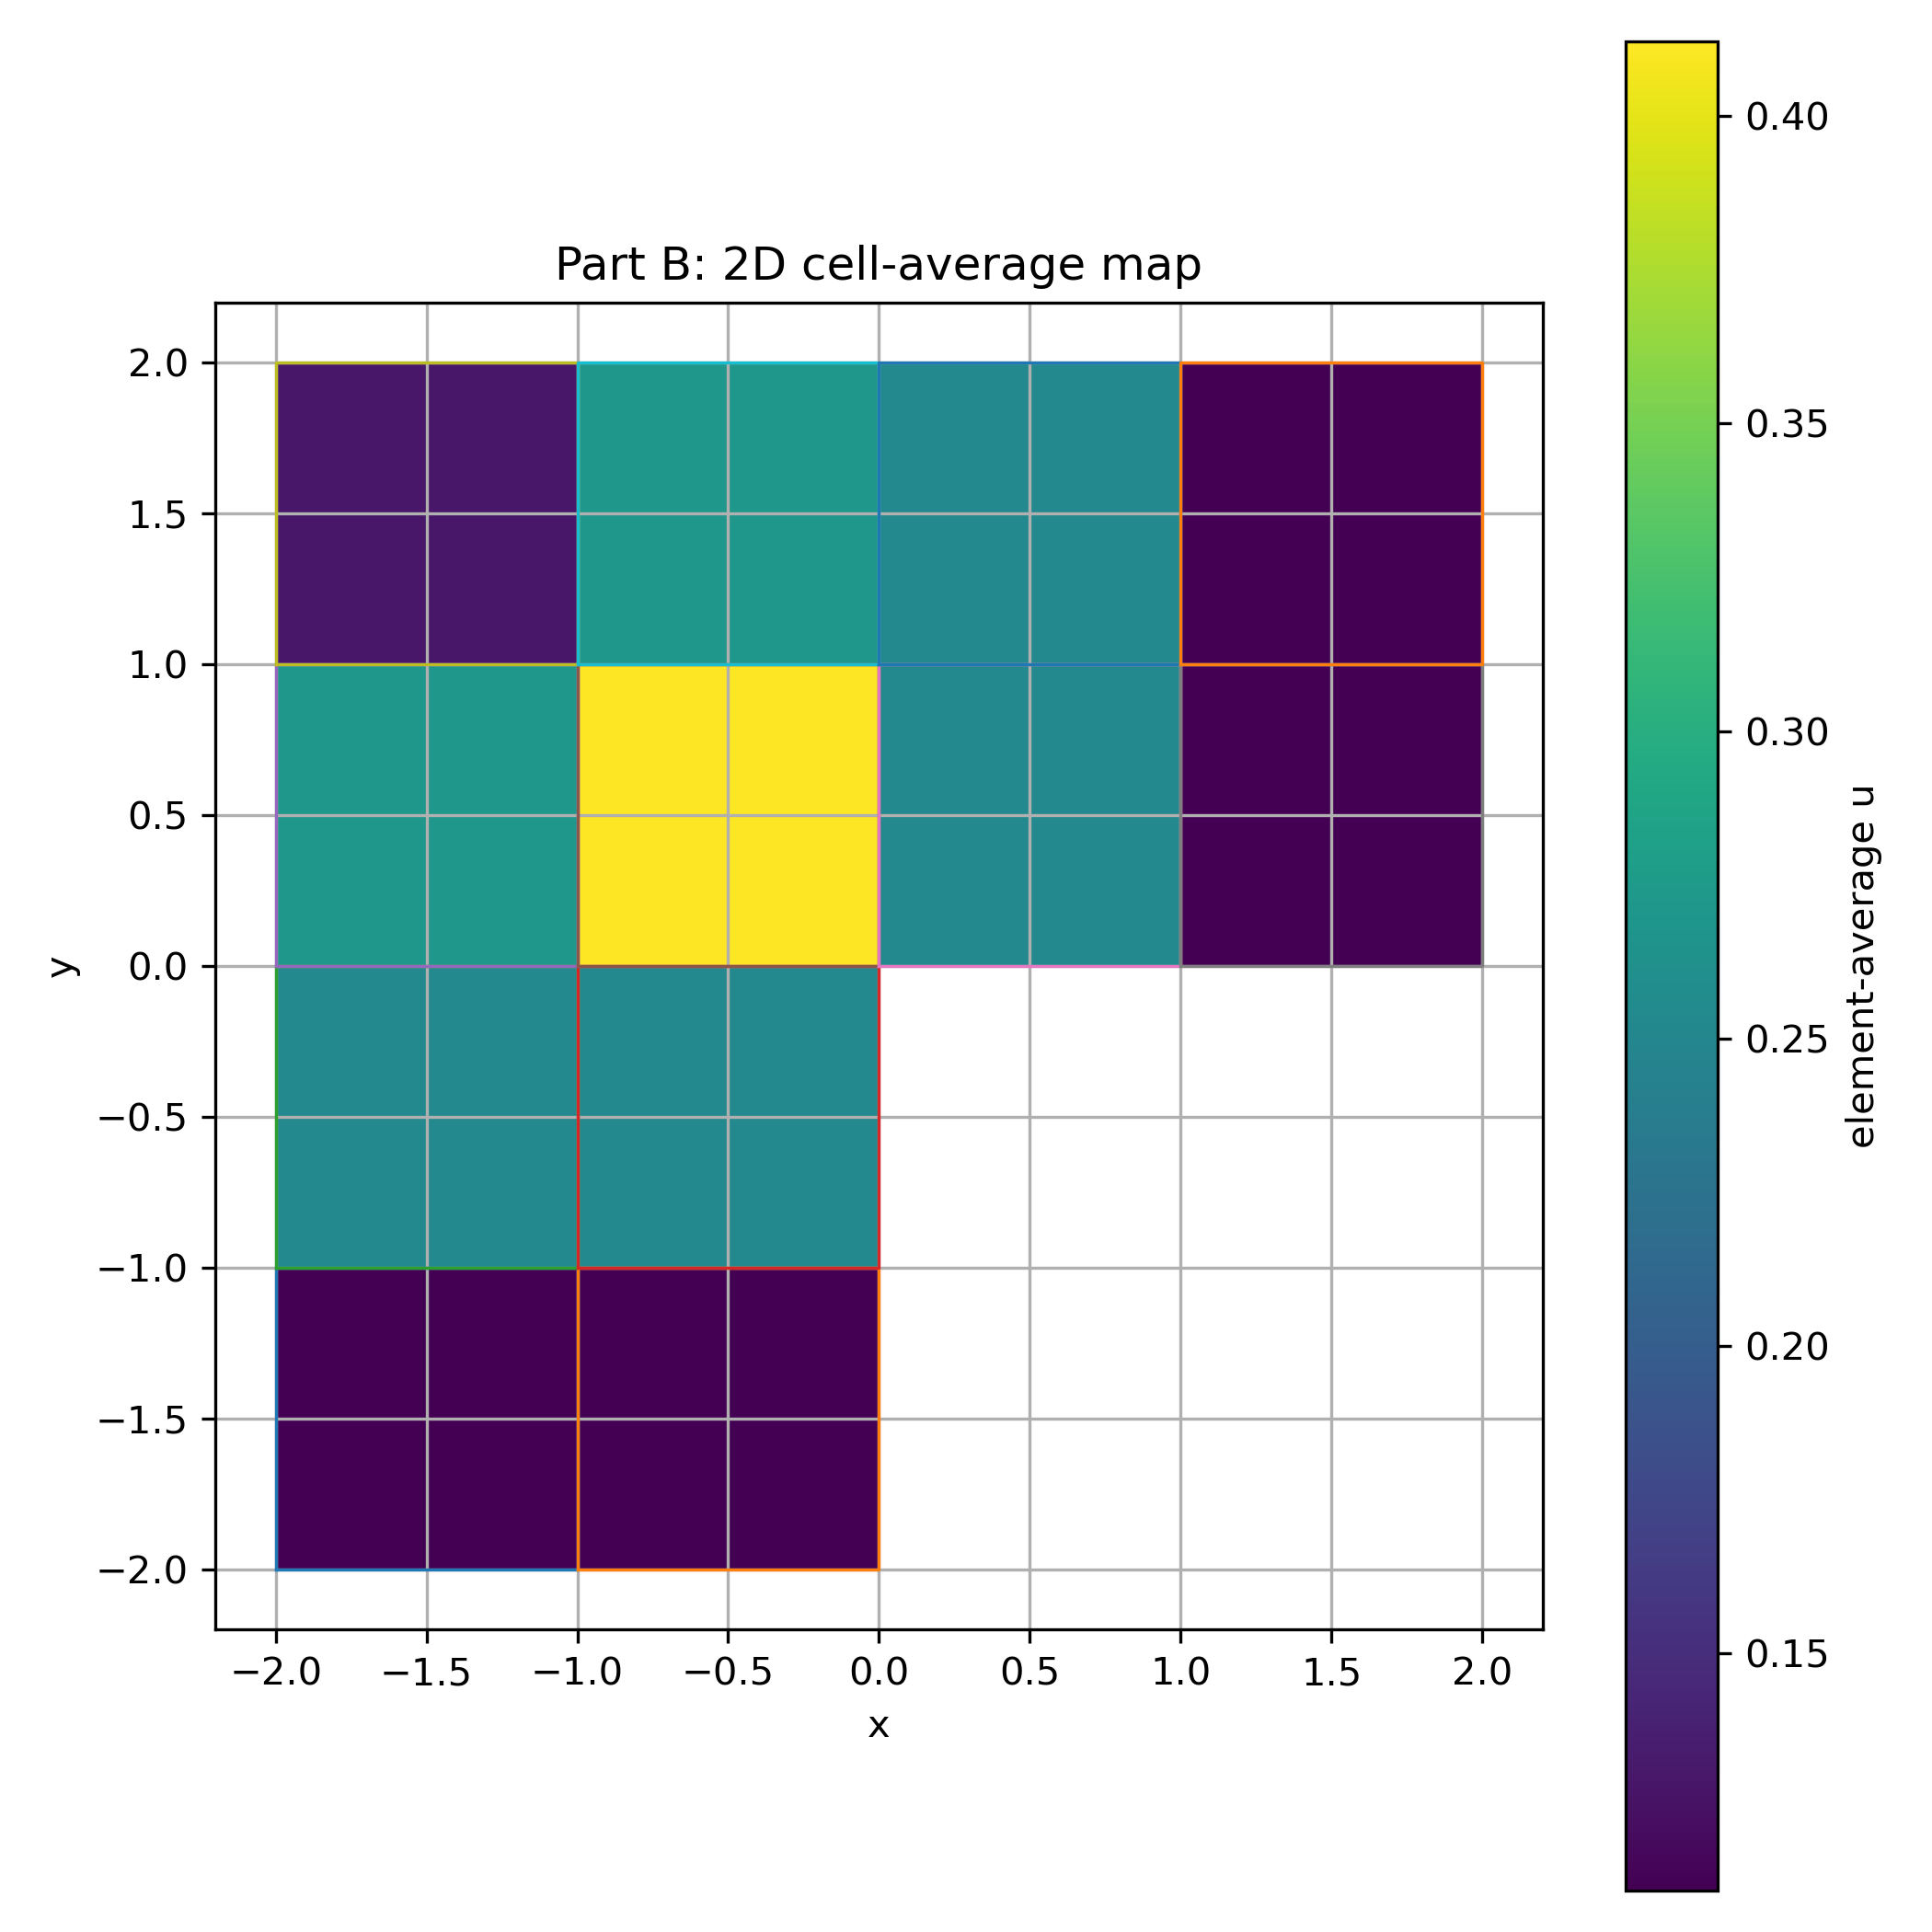
\includegraphics[width=0.80\textwidth]{images/partB_2D_cell_average_map.png}
\caption{Part B two-dimensional cell-average map of the computed scalar field.}
\label{fig:partb_cell_map}
\end{figure}

\subsection{Three-Dimensional Nodal Plot}

\begin{figure}[H]
\centering
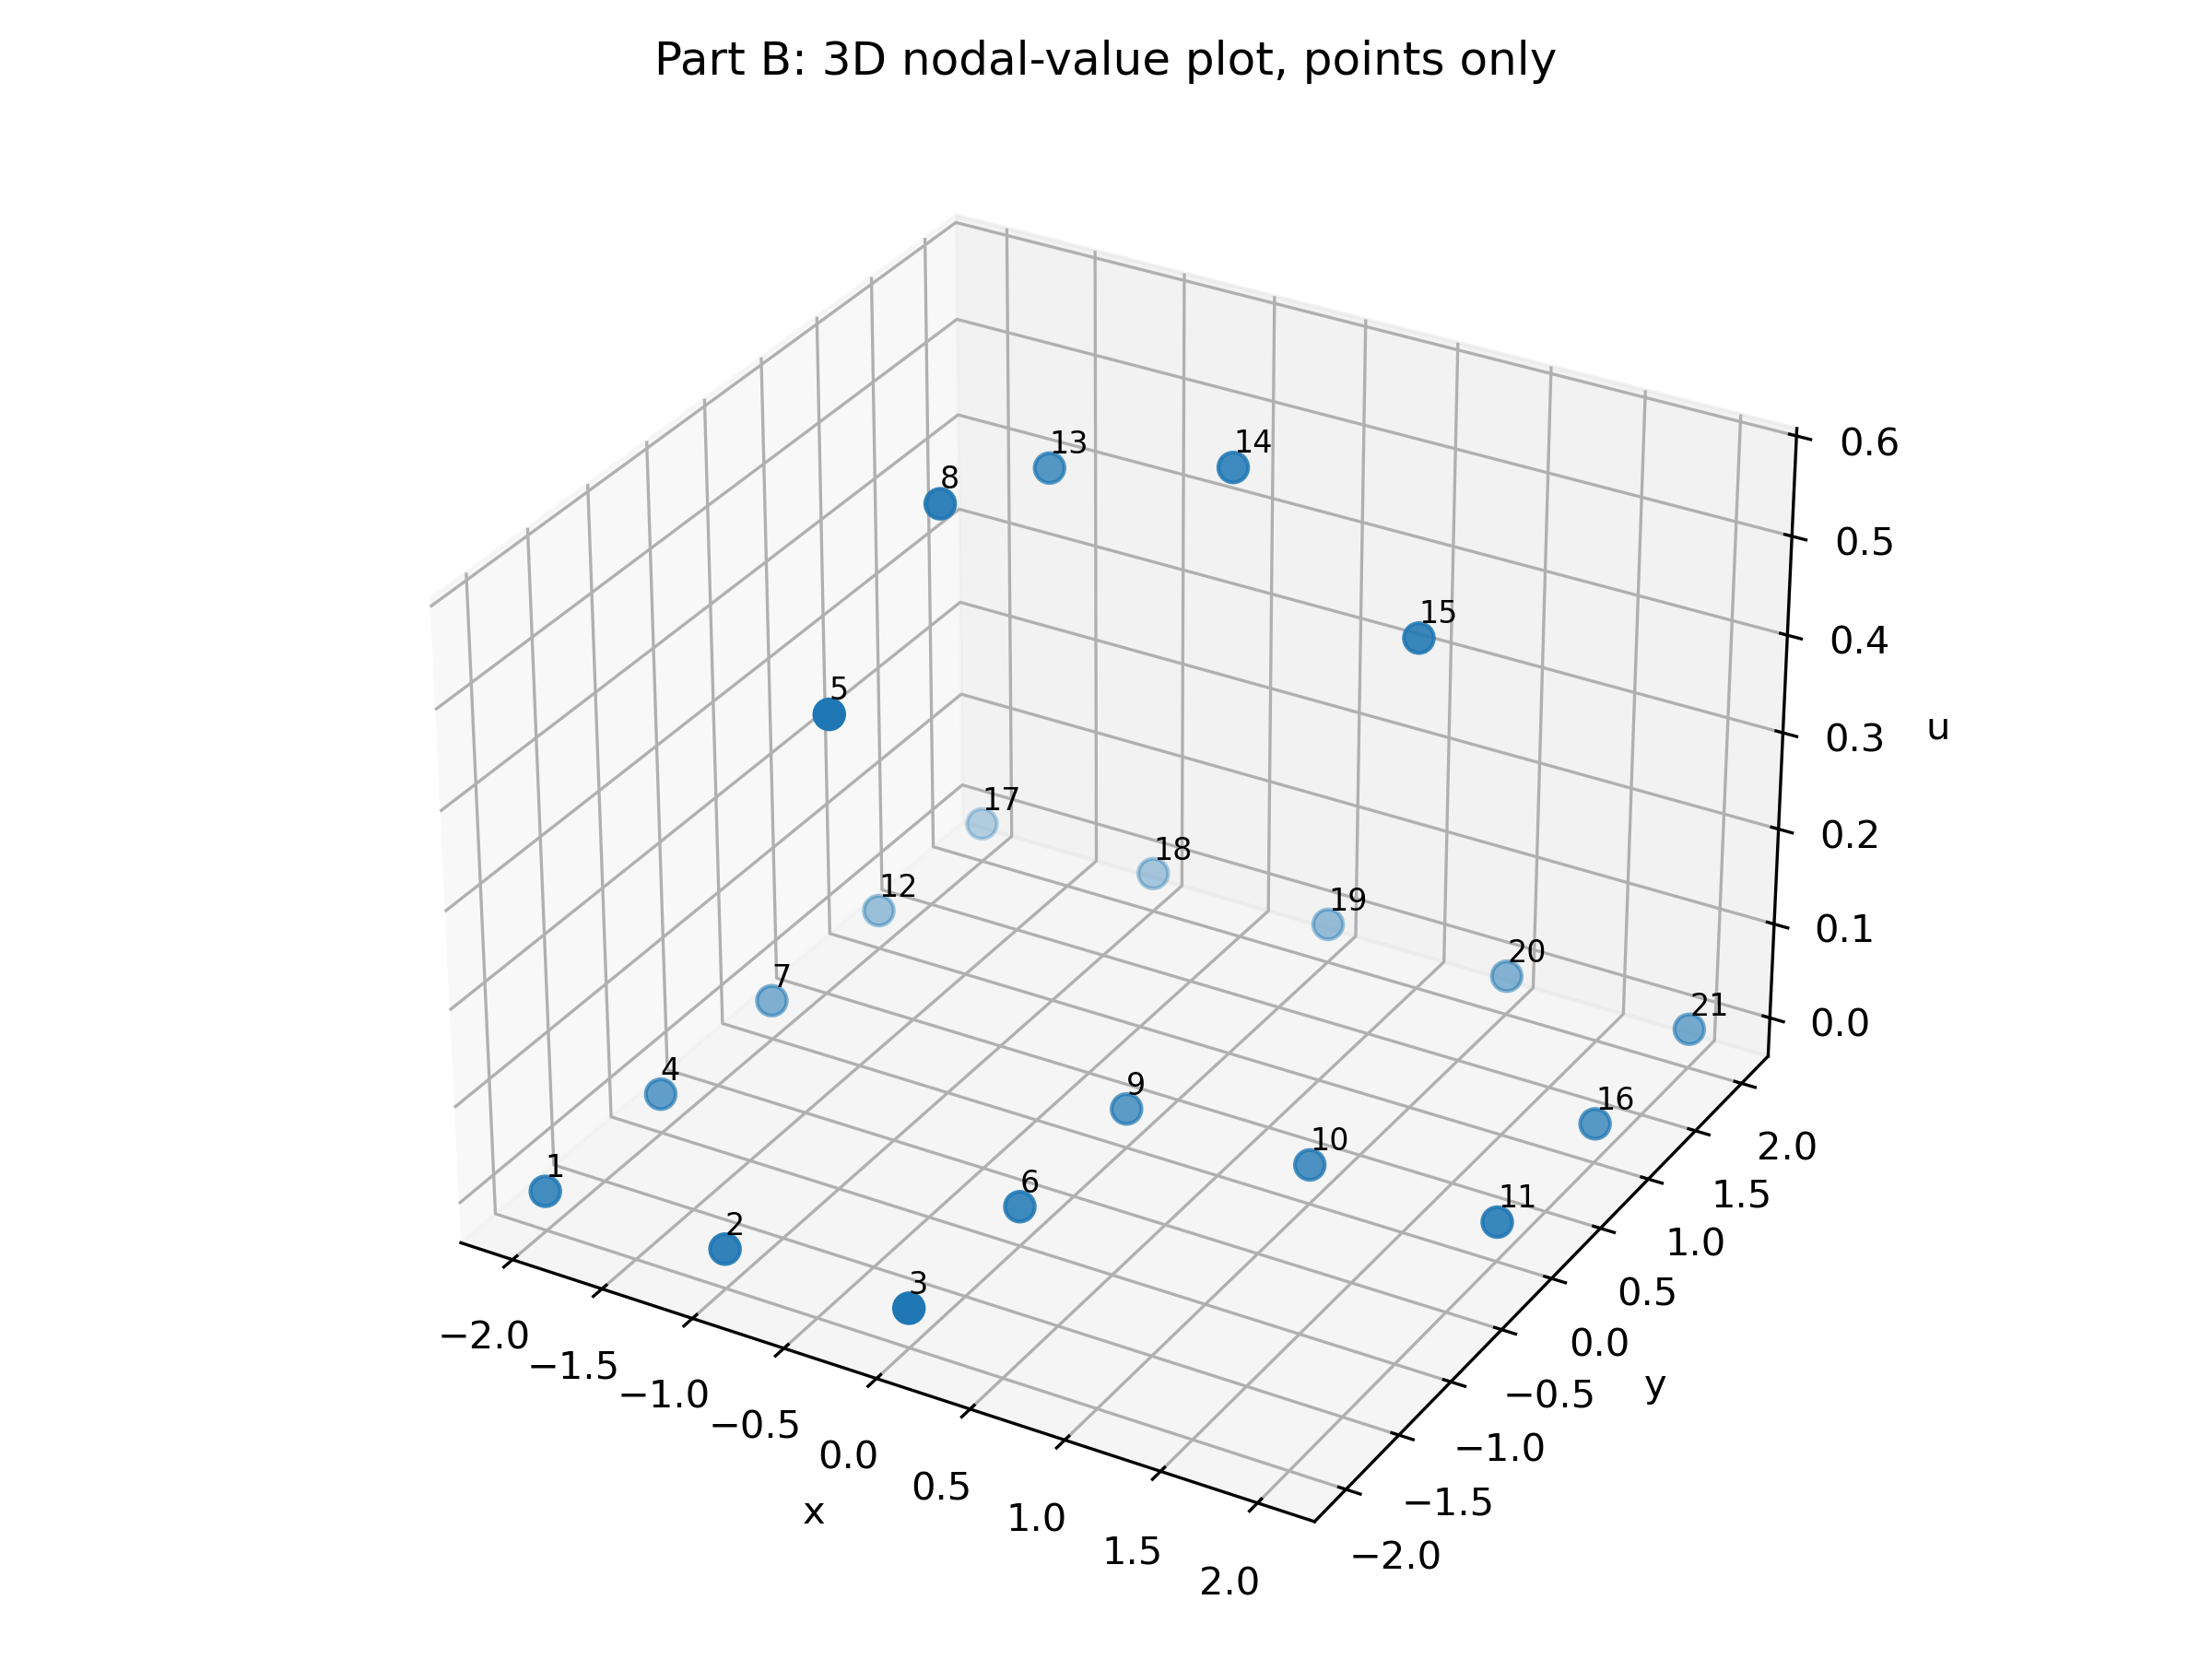
\includegraphics[width=0.80\textwidth]{images/partB_3D_points_only.png}
\caption{Part B three-dimensional nodal-value plot shown as a points-only surface.}
\label{fig:partb_3d}
\end{figure}

\subsection{Gradient Results}

For bilinear rectangular elements, the gradient is not constant inside an element. It is evaluated using
\begin{equation}
    u_{,x}=\sum_{i=1}^4 u_i\frac{\partial N_i}{\partial x},
    \qquad
    u_{,y}=\sum_{i=1}^4 u_i\frac{\partial N_i}{\partial y}.
\end{equation}

At $(-0.5,0)$, two adjacent rectangles give
\begin{align}
    \grad u^{-} &= \vect{-0.566038\\0.060142}
    =\vect{-30/53\\51/848},\\
    \grad u^{+} &= \vect{-0.566038\\0.258255}
    =\vect{-30/53\\219/848},\\
    \grad u_{\mathrm{avg}} &= \vect{-0.566038\\0.159198}
    =\vect{-30/53\\135/848}.
\end{align}

At $(0,0.5)$, two adjacent rectangles give
\begin{align}
    \grad u^{-} &= \vect{-0.258255\\0.566038}
    =\vect{-219/848\\30/53},\\
    \grad u^{+} &= \vect{-0.060142\\0.566038}
    =\vect{-51/848\\30/53},\\
    \grad u_{\mathrm{avg}} &= \vect{-0.159198\\0.566038}
    =\vect{-135/848\\30/53}.
\end{align}

\subsection{Flux Results}

Since bilinear rectangular-element gradients vary with position, the boundary flux was evaluated at the midpoint of each boundary segment.

On $x=2$,
\begin{equation}
    n=\vect{1\\0},
\end{equation}
so at the midpoints of the two boundary segments,
\begin{equation}
    k\grad u\cdot n=-0.222877=-\frac{189}{848}.
\end{equation}

On $y=-2$,
\begin{equation}
    n=\vect{0\\-1},
\end{equation}
so at the midpoints of the two boundary segments,
\begin{equation}
    k\grad u\cdot n=-0.222877=-\frac{189}{848}.
\end{equation}

\section{Comparison of Triangular and Rectangular Results}

The triangular and rectangular solutions give different nodal patterns:
\begin{table}[H]
\centering
\caption{Comparison of free-node solutions.}
\begin{tabular}{rrrr}
\toprule
Node & Coordinate & Part A: Triangles & Part B: Rectangles \\
\midrule
5  & $(-1,-1)$ & 0.435897 & 0.445755 \\
8  & $(-1,0)$  & 0.410256 & 0.566038 \\
13 & $(-1,1)$  & 0.538462 & 0.516509 \\
14 & $(0,1)$   & 0.410256 & 0.566038 \\
15 & $(1,1)$   & 0.435897 & 0.445755 \\
\bottomrule
\end{tabular}
\end{table}

For this particular coarse discretization, the triangular-element solution appears more physically reasonable. The triangular solution gives the maximum value at node 13, \(u_{13}=0.5385\), which lies near the interior of the L-shaped domain and away from most of the zero-Dirichlet boundaries. In contrast, the bilinear rectangular solution gives its largest values at nodes 8 and 14, \(u_8=u_{14}=0.5660\), while \(u_{13}=0.5165\). This shift of the maximum is less intuitive for the present coarse mesh.

However, this conclusion should not be generalized. Bilinear rectangular elements have a richer interpolation field than linear triangular elements, so they may become more accurate under refinement or in smoother rectangular regions. The L-shaped domain also contains a re-entrant corner with interior angle \(3\pi/2\), which produces singular gradient behavior in the true solution. Therefore, neither coarse discretization can accurately resolve the local flux/gradient field near the re-entrant corner. A rigorous accuracy comparison would require an exact solution, a refined-mesh reference solution, or a mesh-convergence study.

Thus, for this specific coarse mesh, the triangular result is preferred because its nodal pattern is more physically plausible, but this is not a universal statement about triangular elements being more accurate than bilinear rectangular elements.

\section{Part C: Discussion of Results}

The triangular and rectangular discretizations solve the same governing problem,

\[
-\Delta u = 1
\]

with homogeneous Dirichlet boundary conditions,

\[
u=0 \quad \text{on } \Gamma .
\]

Therefore, both solutions show the expected qualitative behavior: all boundary nodes remain zero, while the interior nodes take positive values. This is physically reasonable for the membrane, torsion, or heat-conduction interpretations of the problem. Since the source term is positive over the domain, the solution rises inside the domain and decreases toward the boundary.

The triangular-element solution gives

\[
u_5=0.4359,\quad
u_8=0.4103,\quad
u_{13}=0.5385,\quad
u_{14}=0.4103,\quad
u_{15}=0.4359.
\]

The maximum occurs at node 13, which is near the interior of the L-shaped region. The triangular approximation is piecewise linear, so the solution surface consists of planar triangular facets. Consequently, the gradient and flux are constant within each triangular element, but may be discontinuous across element boundaries.

The bilinear rectangular solution gives approximately

\[
u_5=0.4458,\quad
u_8=0.5660,\quad
u_{13}=0.5165,\quad
u_{14}=0.5660,\quad
u_{15}=0.4458.
\]

This solution has a different nodal pattern, with larger values at nodes 8 and 14. The rectangular elements use bilinear interpolation, so the solution varies bilinearly inside each element. Unlike the triangular case, the gradient and flux are not constant inside a rectangular element; they vary with position. This explains why the rectangular flux expressions are coordinate-dependent, while the triangular fluxes are constant over each adjacent triangular element.

A key feature of this problem is the re-entrant corner of the L-shaped domain. The interior angle at the re-entrant corner is \(3\pi/2\), and such corners are known to produce singular gradient behavior in elliptic boundary-value problems. The solution \(u\) itself remains finite, but the gradient and flux field can become very large near the corner. Therefore, neither of the coarse meshes used in this assignment should be expected to capture the local gradient behavior accurately near the re-entrant corner. This is especially important when interpreting the flux results.

The global balance condition also provides a useful consistency check. Since

\[
-\Delta u = 1,
\]

integrating over the domain gives

\[
-\int_{\Gamma} \nabla u \cdot n \, d\Gamma
=
\int_{\Omega} 1\,d\Omega
=
|\Omega|.
\]

The L-shaped domain consists of 12 unit square cells, so

\[
|\Omega|=12.
\]

Thus, the total physical outward flux,

\[
q_n=-\nabla u\cdot n,
\]

should balance the total source and integrate to approximately 12 over the full boundary. The fluxes reported in this assignment are only evaluated along selected boundary lines, \(x=2\) and \(y=-2\), so they do not by themselves represent the full boundary balance. A complete flux-reaction recovery over all boundary segments would be needed for a full conservation check.

Overall, the results show that element type and interpolation choice strongly affect the numerical solution on coarse meshes. For this specific discretization, the triangular solution appears more physically plausible because the peak occurs at node 13, near the interior of the L-shaped domain. However, this conclusion is limited by the coarse mesh and by the unresolved re-entrant-corner singularity. A more rigorous accuracy comparison would require mesh refinement or comparison with a benchmark solution.

\section{Conclusion}

Both the triangular and rectangular discretizations successfully produce finite element approximations for the same L-shaped Poisson problem. The triangular discretization gives a peak value at node 13, while the bilinear rectangular discretization gives peak values at nodes 8 and 14. The difference demonstrates that element type and interpolation assumptions can significantly affect results on coarse meshes.

The triangular solution is preferred for this specific assignment because its nodal pattern is more physically intuitive for the L-shaped domain. Nevertheless, the conclusion is limited by the coarseness of the mesh. A more rigorous comparison would require mesh refinement or comparison with a benchmark solution.

\end{document}
